%%%   K A L E V A L A   %%%

\documentclass[oneside]{book}

\usepackage[paperwidth=130mm, paperheight=297mm]{geometry}
\usepackage[utf8]{inputenc}
\usepackage[T1]{fontenc}
\usepackage[finnish]{babel}
\usepackage{yfonts}
\usepackage{graphicx}
\usepackage[names,dvipsnames]{xcolor}
\usepackage{fancyhdr}
\usepackage{sectsty}
\usepackage{lettrine}

\title{\textfrak{Kalevala}}
\author{\textfrak{koonnut:\\Elias Lönnrot}}

\pagestyle{fancy}

\fancyhf{} % Sets both header and footer to nothing
\renewcommand{\headrulewidth}{0pt} % Line a the header invisible
% Define {fancyhdr} headers and footers
\lhead{}
\chead{}
\rhead{}
\lfoot{}
\cfoot{\textbf{\color{BrickRed}{\oldstylenums{\thepage}}}}
\rfoot{}

% Redefine the plain page style
\fancypagestyle{plain}{%
  \fancyhf{}%
  \fancyfoot[C]{\textbf{\color{BrickRed}{\oldstylenums{\thepage}}}}%
  \renewcommand{\headrulewidth}{0pt}% Line at the header invisible
}

% Font for dropped caps
\input MorrisIn.fd
\renewcommand*\initfamily{\usefont{U}{MorrisIn}{xl}{n}}

% Colored initial
\newcommand{\colorini}[2]{\lettrine[lines=3]{\textcolor{BrickRed}{\initfamily{#1}}}{#2}}

% Define chapter title
\allsectionsfont{\color{BrickRed}\textfrak}

\begin{document}

\begin{titlepage}
    \centering
   
    \textcolor{BrickRed}{\rule{\textwidth}{1.6pt}\vspace*{-\baselineskip}\vspace*{2pt}
    \rule{\textwidth}{0.4pt}}\\[\baselineskip]
    \Huge{\textfrak{Kalevala}}
    \textcolor{BrickRed}{\rule{\textwidth}{0.4pt}\vspace*{-\baselineskip}\vspace{3.2pt}
    \rule{\textwidth}{1.6pt}}\\[\baselineskip]

    \vspace*{2\baselineskip}
    
    \LARGE{\textfrak{Elias: Lönnrot}}
    
    \vfill
    {\scshape year} \\
    {\large THE PUBLISHER}\par
	\end{titlepage}
	
	\vspace*{5cm}
	\begin{center}
		
\includegraphics[width=0.20\textwidth]{./img/k.pdf}
	\end{center}
		
	\begin{figure}[ht]
		\centering
			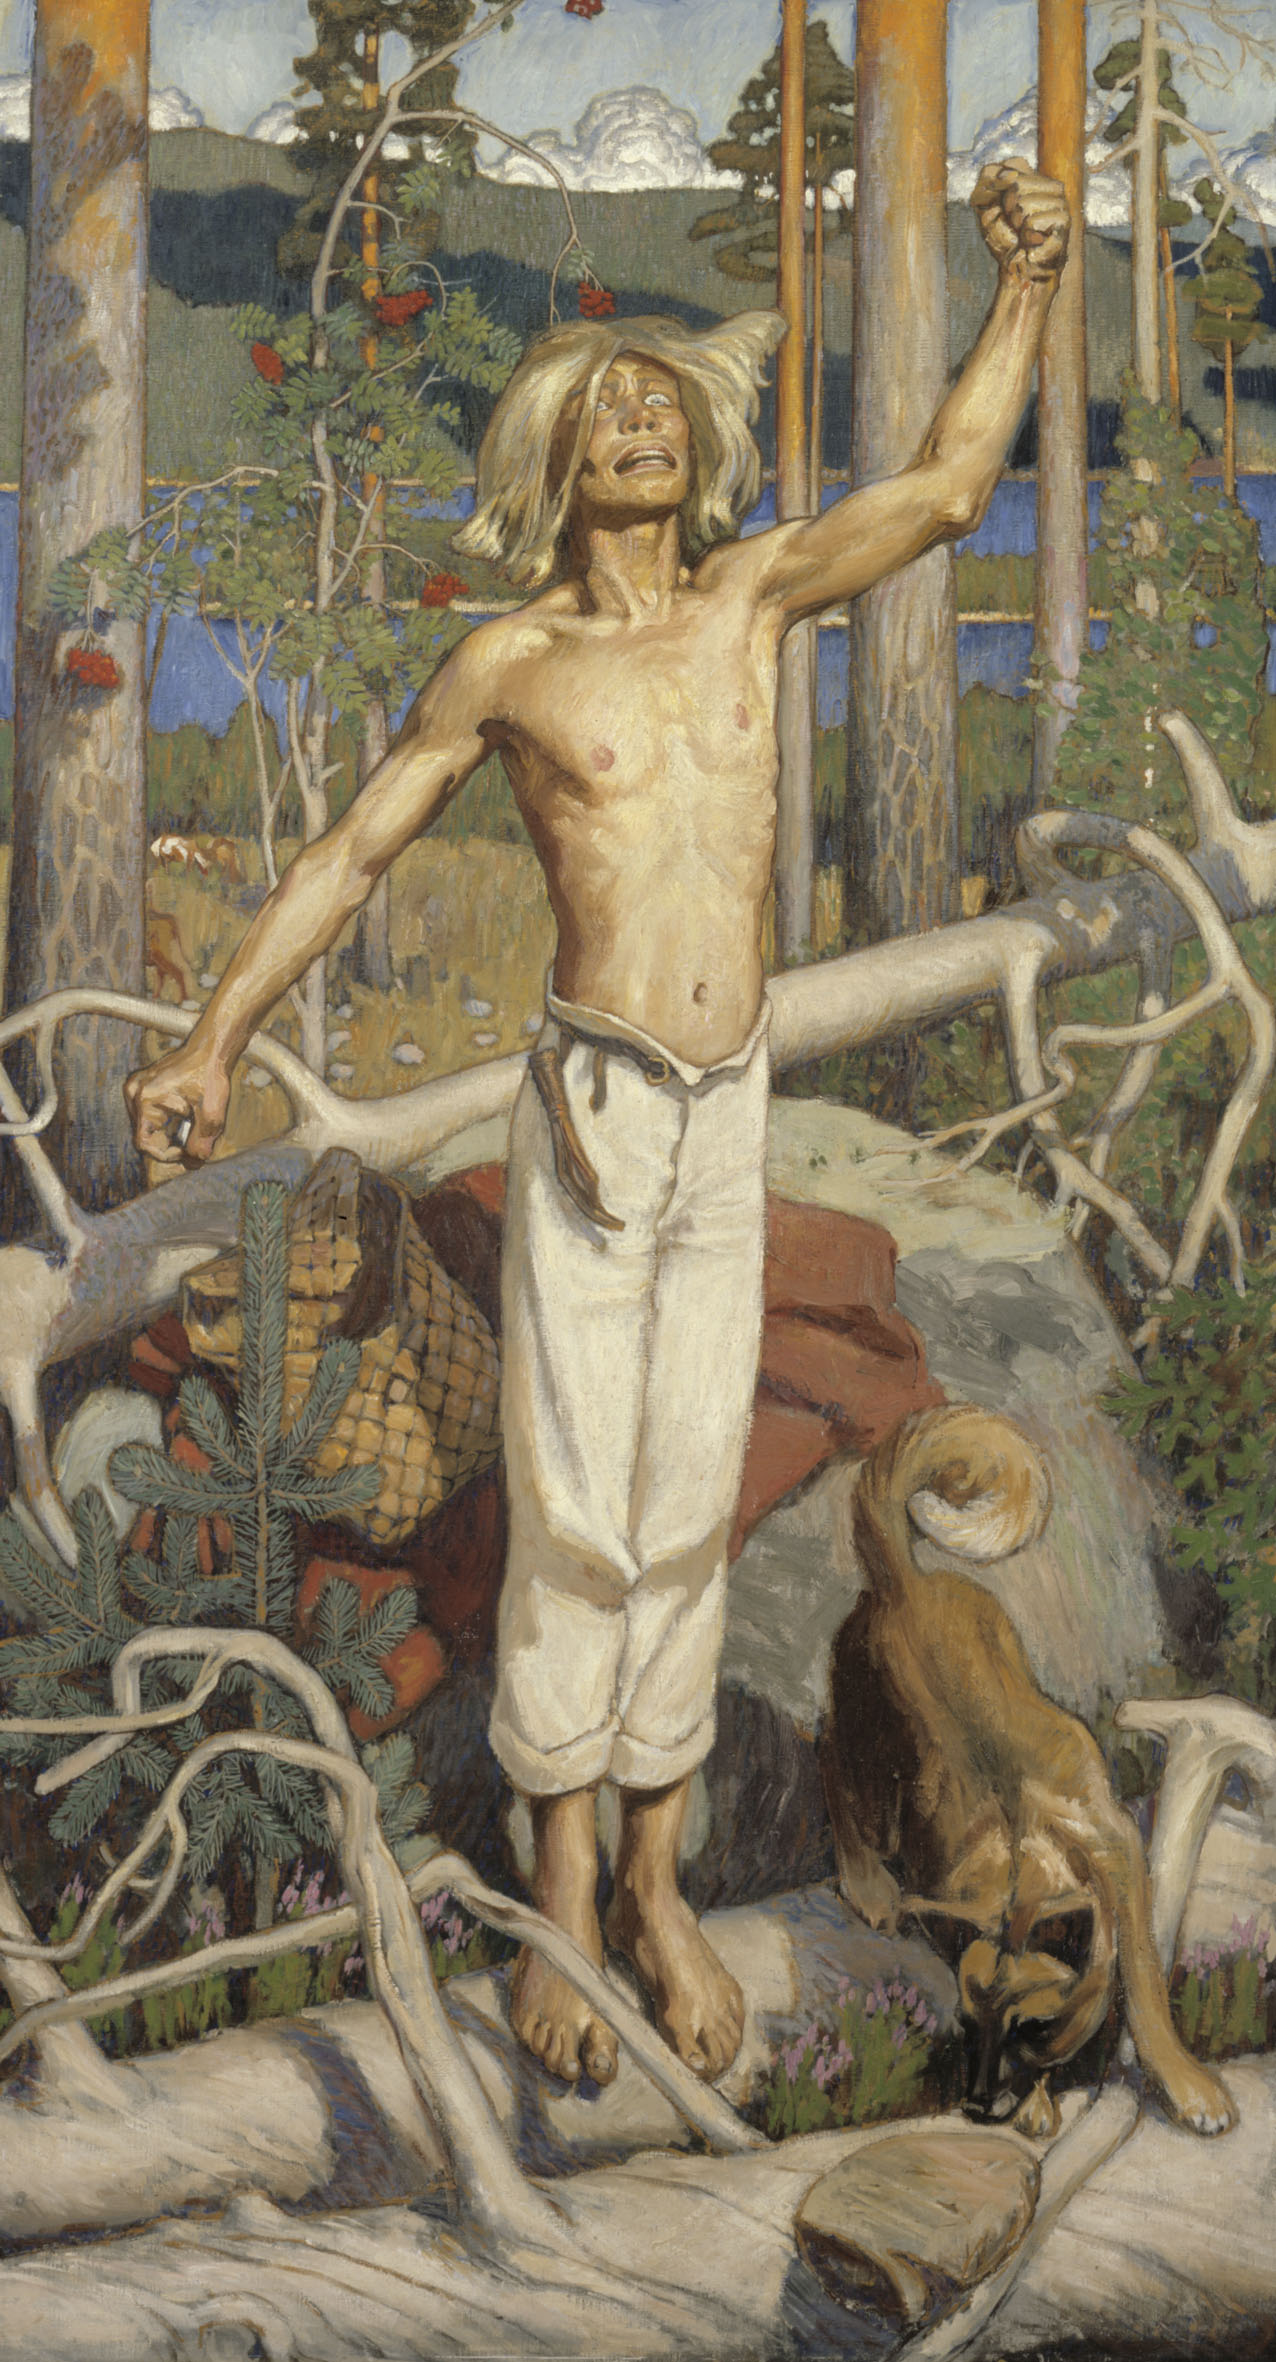
\includegraphics[width=1.00\textwidth]{./img/kullervo.png}
%		\caption{Kullervon kirous Akseli Gallen-Kallela}
%		\label{fig:kullervo}
	\end{figure}
	
	% Ensimmäinen runo

\chapter*{Ensimmäinen Runo}

\colorini{M}{ieleni minun tekevi}, aivoni ajattelevi          \\
lähteäni laulamahan, saa'ani sanelemahan,				          	\\	
sukuvirttä suoltamahan, lajivirttä laulamahan.              \\
Sanat suussani sulavat, puhe'et putoelevat,                 \\
kielelleni kerkiävät, hampahilleni hajoovat.                \\
                                                            \\
Veli kulta, veikkoseni, kaunis kasvinkumppalini!            \\
Lähe nyt kanssa laulamahan, saa kera sanelemahan            \\
yhtehen yhyttyämme, kahta'alta käytyämme!                   \\
Harvoin yhtehen yhymme, saamme toinen toisihimme            \\
näillä raukoilla rajoilla, poloisilla Pohjan mailla.        \\
                                                            \\
Lyökämme käsi kätehen, sormet sormien lomahan,              \\
lauloaksemme hyviä, parahia pannaksemme,                    \\
kuulla noien kultaisien, tietä mielitehtoisien,             \\
nuorisossa nousevassa, kansassa kasuavassa:                 \\
noita saamia sanoja, virsiä virittämiä                      \\
vyöltä vanhan Väinämöisen, alta ahjon Ilmarisen,            \\
päästä kalvan Kaukomielen, Joukahaisen jousen tiestä,       \\
Pohjan peltojen periltä, Kalevalan kankahilta.              \\
                                                            \\
Niit' ennen isoni lauloi kirvesvartta vuollessansa;         \\
niitä äitini opetti väätessänsä värttinätä,                 \\
minun lasna lattialla eessä polven pyöriessä,               \\
maitopartana pahaisna, piimäsuuna pikkaraisna.              \\
Sampo ei puuttunut sanoja eikä Louhi luottehia:             \\
vanheni sanoihin sampo, katoi Louhi luottehisin,            \\
virsihin Vipunen kuoli, Lemminkäinen leikkilöihin.          \\
                                                            \\
Viel' on muitaki sanoja, ongelmoita oppimia:                \\
tieohesta tempomia, kanervoista katkomia,                   \\
risukoista riipomia, vesoista vetelemiä,                    \\
päästä heinän hieromia, raitiolta ratkomia,                 \\
paimenessa käyessäni, lasna karjanlaitumilla,               \\
metisillä mättähillä, kultaisilla kunnahilla,               \\
mustan Muurikin jälessä, Kimmon kirjavan keralla.           \\
                                                            \\
Vilu mulle virttä virkkoi, sae saatteli runoja.             \\
Virttä toista tuulet toivat, meren aaltoset ajoivat.        \\
Linnut liitteli sanoja, puien latvat lausehia.              \\
                                                            \\
Ne minä kerälle käärin, sovittelin sommelolle.              \\
Kerän pistin kelkkahani, sommelon rekoseheni;               \\
ve'in kelkalla kotihin, rekosella riihen luoksi;            \\
panin aitan parven päähän vaskisehen vakkasehen.            \\
                                                            \\
Viikon on virteni vilussa, kauan kaihossa sijaisnut.        \\
Veänkö vilusta virret, lapan laulut pakkasesta,             \\
tuon tupahan vakkaseni, rasian rahin nenähän,               \\
alle kuulun kurkihirren, alle kaunihin katoksen,            \\
aukaisen sanaisen arkun, virsilippahan viritän,             \\
kerittelen pään kerältä, suorin solmun sommelolta?          \\
                                                            \\
Niin laulan hyvänki virren, kaunihinki kalkuttelen          \\
ruoalta rukihiselta, oluelta ohraiselta.                    \\
Kun ei tuotane olutta, tarittane taarivettä,                \\
laulan suulta laihemmalta, vetoselta vierettelen            \\
tämän iltamme iloksi, päivän kuulun kunniaksi,              \\
vaiko huomenen huviksi, uuen aamun alkeheksi.               \\
                                                            \\
Noin kuulin saneltavaksi, tiesin virttä tehtäväksi:         \\
yksin meillä yöt tulevat, yksin päivät valkeavat;           \\
yksin syntyi Väinämöinen, ilmestyi ikirunoja                \\
kapehesta kantajasta, Ilmattaresta emosta.                  \\
                                                            \\
Olipa impi, ilman tyttö, kave luonnotar korea.              \\
Piti viikoista pyhyyttä, iän kaiken impeyttä                \\
ilman pitkillä pihoilla, tasaisilla tanterilla.             \\
                                                            \\
Ikävystyi aikojansa, ouostui elämätänsä,                    \\
aina yksin ollessansa, impenä eläessänsä                    \\
ilman pitkillä pihoilla, avaroilla autioilla.               \\
                                                            \\
Jop' on astuiksen alemma, laskeusi lainehille,              \\
meren selvälle selälle, ulapalle aukealle.                  \\
Tuli suuri tuulen puuska, iästä vihainen ilma;              \\
meren kuohuille kohotti, lainehille laikahutti.             \\
                                                            \\
Tuuli neittä tuuitteli, aalto impeä ajeli                   \\
ympäri selän sinisen, lakkipäien lainehien:                 \\
tuuli tuuli kohtuiseksi, meri paksuksi panevi.              \\
                                                            \\
Kantoi kohtua kovoa, vatsantäyttä vaikeata                  \\
vuotta seitsemän satoa, yheksän yrön ikeä;                  \\
eikä synny syntyminen, luovu luomatoin sikiö.               \\
                                                            \\
Vieri impi veen emona. Uipi iät, uipi lännet,               \\
uipi luotehet, etelät, uipi kaikki ilman rannat             \\
tuskissa tulisen synnyn, vatsanvaivoissa kovissa;           \\
eikä synny syntyminen, luovu luomatoin sikiö.               \\
                                                            \\
Itkeä hyryttelevi; sanan virkkoi, noin nimesi:              \\
"Voi poloinen, päiviäni, lapsi kurja, kulkuani!             \\
Jo olen joutunut johonki: iäkseni ilman alle,               \\
tuulen tuuiteltavaksi, aaltojen ajeltavaksi                 \\
näillä väljillä vesillä, lake'illa lainehilla!              \\
                                                            \\
"Parempi olisi ollut ilman impenä eleä,                     \\
kuin on nyt tätä nykyä vierähellä veen emona:               \\
vilu tääll' on ollakseni, vaiva värjätelläkseni,            \\
aalloissa asuakseni, veessä vierielläkseni.                 \\
                                                            \\
"Oi Ukko, ylijumala, ilman kaiken kannattaja!               \\
Tule tänne tarvittaissa, käy tänne kutsuttaessa!            \\
Päästä piika pintehestä, vaimo vatsanvääntehestä!           \\
Käy pian, välehen jou'u, välehemmin tarvitahan!"            \\
                                                            \\
Kului aikoa vähäisen, pirahteli pikkaraisen.                \\
Tuli sotka, suora lintu; lenteä lekuttelevi                 \\
etsien pesän sijoa, asuinmaata arvaellen.                   \\
                                                            \\
Lenti iät, lenti lännet, lenti luotehet, etelät.            \\
Ei löyä tiloa tuota, paikkoa pahintakana,                   \\
kuhun laatisi pesänsä, ottaisi olosijansa.                  \\
                                                            \\
Liitelevi, laatelevi; arvelee, ajattelevi:                  \\
"Teenkö tuulehen tupani, aalloillen asuinsijani?            \\
Tuuli kaatavi tupasen, aalto vie asuinsijani."              \\
                                                            \\
Niin silloin ve'en emonen, veen emonen, ilman impi,         \\
nosti polvea merestä, lapaluuta lainehesta                  \\
sotkalle pesän sijaksi, asuinmaaksi armahaksi.              \\
                                                            \\
Tuo sotka, sorea lintu, liiteleikse, laateleikse.           \\
Keksi polven veen emosen sinerväisellä selällä;             \\
luuli heinämättähäksi, tuoreheksi turpeheksi.               \\
                                                            \\
Lentelevi, liitelevi, päähän polven laskeuvi.               \\
Siihen laativi pesänsä, muni kultaiset munansa:             \\
kuusi kultaista munoa, rautamunan seitsemännen.             \\
                                                            \\
Alkoi hautoa munia, päätä polven lämmitellä.                \\
Hautoi päivän, hautoi toisen, hautoi kohta kolmannenki.     \\
                                                            \\
Jopa tuosta veen emonen, veen emonen, ilman impi,           \\
tuntevi tulistuvaksi, hipiänsä hiiltyväksi;                 \\
luuli polvensa palavan, kaikki suonensa sulavan.            \\
                                                            \\
Vavahutti polveansa, järkytti jäseniänsä:                   \\
munat vierähti vetehen, meren aaltohon ajaikse;             \\
karskahti munat muruiksi, katkieli kappaleiksi.             \\
                                                            \\
Ei munat mutahan joua, siepalehet veen sekahan.             \\
Muuttuivat murut hyviksi, kappalehet kaunoisiksi:           \\
munasen alainen puoli alaiseksi maaemäksi,                  \\
munasen yläinen puoli yläiseksi taivahaksi;                 \\
yläpuoli ruskeaista päivöseksi paistamahan,                 \\
yläpuoli valkeaista, se kuuksi kumottamahan;                \\
mi munassa kirjavaista, ne tähiksi taivahalle,              \\
mi munassa mustukaista, nepä ilman pilvilöiksi.             \\
                                                            \\
Ajat eellehen menevät, vuoet tuota tuonnemmaksi             \\
uuen päivän paistaessa, uuen kuun kumottaessa.              \\
Aina uipi veen emonen, veen emonen, ilman impi,             \\
noilla vienoilla vesillä, utuisilla lainehilla,             \\
eessänsä vesi vetelä, takanansa taivas selvä.               \\
                                                            \\
Jo vuonna yheksäntenä, kymmenentenä kesänä                  \\
nosti päätänsä merestä, kohottavi kokkoansa.                \\
Alkoi luoa luomiansa, saautella saamiansa                   \\
selvällä meren selällä, ulapalla aukealla.                  \\
                                                            \\
Kussa kättä käännähytti, siihen niemet siivoeli;            \\
kussa pohjasi jalalla, kalahauat kaivaeli;                  \\
kussa ilman kuplistihe, siihen syöverit syventi.            \\
                                                            \\
Kylin maahan kääntelihe: siihen sai sileät rannat;          \\
jaloin maahan kääntelihe: siihen loi lohiapajat;            \\
pä'in päätyi maata vasten: siihen laitteli lahelmat.        \\
                                                            \\
Ui siitä ulomma maasta, seisattelihe selälle:               \\
luopi luotoja merehen, kasvatti salakaria                   \\
laivan laskemasijaksi, merimiesten pään menoksi.            \\
                                                            \\
Jo oli saaret siivottuna, luotu luotoset merehen,           \\
ilman pielet pistettynä, maat ja manteret sanottu,          \\
kirjattu kivihin kirjat, veetty viivat kallioihin.          \\
Viel' ei synny Väinämöinen, ilmau ikirunoja.                \\
                                                            \\
Vaka vanha Väinämöinen kulki äitinsä kohussa                \\
kolmekymmentä keseä, yhen verran talviaki,                  \\
noilla vienoilla vesillä, utuisilla lainehilla.             \\
                                                            \\
Arvelee, ajattelevi, miten olla, kuin eleä                  \\
pimeässä piilossansa, asunnossa ahtahassa,                  \\
kuss' ei konsa kuuta nähnyt eikä päiveä havainnut.          \\
                                                            \\
Sanovi sanalla tuolla, lausui tuolla lausehella:            \\
"Kuu, keritä, päivyt, päästä, otava, yhä opeta              \\
miestä ouoilta ovilta, veräjiltä vierahilta,                \\
näiltä pieniltä pesiltä, asunnoilta ahtahilta!              \\
Saata maalle matkamiestä, ilmoillen inehmon lasta,          \\
kuuta taivon katsomahan, päiveä ihoamahan,                  \\
otavaista oppimahan, tähtiä tähyämähän!"                    \\
                                                            \\
Kun ei kuu kerittänynnä eikä päivyt päästänynnä,            \\
ouosteli aikojansa, tuskastui elämätänsä:                   \\
liikahutti linnan portin sormella nimettömällä,             \\
lukon luisen luikahutti vasemmalla varpahalla;              \\
tuli kynsin kynnykseltä, polvin porstuan ovelta.            \\
                                                            \\
Siitä suistui suin merehen, käsin kääntyi lainehesen;       \\
jääpi mies meren varahan, uros aaltojen sekahan.            \\
                                                            \\
Virui siellä viisi vuotta, sekä viisi jotta kuusi,          \\
vuotta seitsemän, kaheksan. Seisottui selälle viimein,      \\
niemelle nimettömälle, manterelle puuttomalle.              \\
                                                            \\
Polvin maasta ponnistihe, käsivarsin käännältihe.           \\
Nousi kuuta katsomahan, päiveä ihoamahan,                   \\
otavaista oppimahan, tähtiä tähyämähän.                     \\
                                                            \\
Se oli synty Väinämöisen, rotu rohkean runojan              \\
kapehesta kantajasta, Ilmattaresta emosta.			        		\\
	% Toinen runo

\chapter*{Toinen Runo}

\colorini{N}{ousi siitä Väinämöinen} jalan kahen kankahalle				\\
saarehen selällisehen, manterehen puuttomahan.                  \\
                                                                \\
Viipyi siitä vuotta monta, aina eellehen eleli                  \\
saaressa sanattomassa, manteressa puuttomassa.                  \\
                                                                \\
Arvelee, ajattelevi, pitkin päätänsä pitävi:                    \\
kenpä maita kylvämähän, toukoja tihittämähän?                   \\
                                                                \\
Pellervoinen, pellon poika, Sampsa poika pikkarainen,           \\
sep' on maita kylvämähän, toukoja tihittämähän!                 \\
                                                                \\
Kylvi maita kyyhätteli, kylvi maita, kylvi soita,               \\
kylvi auhtoja ahoja, panettavi paasikoita.                      \\
                                                                \\
Mäet kylvi männiköiksi, kummut kylvi kuusikoiksi,               \\
kankahat kanervikoiksi, notkot nuoriksi vesoiksi.               \\
                                                                \\
Noromaille koivut kylvi, lepät maille leyhke'ille,              \\
tuomet kylvi tuorehille, raiat maille raikkahille,              \\
pihlajat pyhille maille, pajut maille paisuville,               \\
katajat karuille maille, tammet virran vieremille.              \\
                                                                \\
Läksi puut ylenemähän, vesat nuoret nousemahan.                 \\
Kasvoi kuuset kukkalatvat, lautui lakkapäät petäjät.            \\
Nousi koivupuut noroilla, lepät mailla leyhke'illä,             \\
tuomet mailla tuorehilla, katajat karuilla mailla,              \\
katajahan kaunis marja, tuomehen hyvä he'elmä.                  \\
                                                                \\
Vaka vanha Väinämöinen kävi tuota katsomahan                    \\
Sampsan siemenen aloa, Pellervoisen kylvämiä.                   \\
Näki puut ylenneheksi, vesat nuoret nousneheksi;                \\
yks' on tammi taimimatta, juurtumatta puu Jumalan.              \\
                                                                \\
Heitti herjan valloillensa, olevillen onnillensa;               \\
vuotti vielä yötä kolme, saman verran päiviäki.                 \\
                                                                \\
Kävi siitä katsomahan viikon päästä viimeistäki:                \\
ei ole tammi kasvanunna, juurtununna puu Jumalan.               \\
                                                                \\
Niin näkevi neljä neittä, viisi veen on morsianta.              \\
Ne oli nurmen niitännässä, kastekorren katkonnassa              \\
nenässä utuisen niemen, päässä saaren terhenisen;               \\
mink' on niitti, sen haravoi, kaikki karhille veteli.           \\
                                                                \\
Tulipa merestä Tursas, uros aalloista yleni.                    \\
Tunki heinäset tulehen, ilmivalkean väkehen;                    \\
ne kaikki poroksi poltti, kypeniksi kyyetteli.                  \\
                                                                \\
Tuli tuhkia läjänen, koko kuivia poroja.                        \\
Saip' on siihen lemmen lehti, lemmen lehti, tammen              \\
terho,                                                          \\
josta kasvoi kaunis taimi, yleni vihanta virpi;                 \\
nousi maasta mansikkaisna, kasvoi kaksihaarukkaisna.            \\
                                                                \\
Ojenteli oksiansa, levitteli lehviänsä.                         \\
Latva täytti taivahalle, lehvät ilmoille levisi:                \\
piätti pilvet juoksemasta, hattarat hasertamasta,               \\
päivän peitti paistamasta, kuuhuen kumottamasta.                \\
                                                                \\
Silloin vanha Väinämöinen arvelee, ajattelevi:                  \\
oisko tammen taittajata, puun sorean sortajata?                 \\
Ikävä inehmon olla, kamala kalojen uia                          \\
ilman päivän paistamatta, kuuhuen kumottamatta.                 \\
                                                                \\
Ei ole sitä urosta eikä miestä urheata,                         \\
joka taisi tammen kaata, satalatvan langettoa.                  \\
                                                                \\
Siitä vanha Väinämöinen itse tuon sanoiksi virkki:              \\
"Kave äiti, kantajani, luonnotar, ylentäjäni!                   \\
Laitapa ve'en väkeä  veessä on väkeä paljo                      \\
tämä tammi taittamahan, puu paha hävittämähän                   \\
eestä päivän paistavaisen, tieltä kuun kumottavaisen!"          \\
                                                                \\
Nousipa merestä miesi, uros aallosta yleni.                     \\
Ei tuo ollut suuren suuri eikä aivan pienen pieni:              \\
miehen peukalon pituinen, vaimon vaaksan korkeuinen.            \\
                                                                \\
Vaski- oli hattu hartioilla, vaskisaappahat jalassa,            \\
vaskikintahat käessä, vaskikirjat kintahissa,                   \\
vaskivyöhyt vyölle vyötty, vaskikirves vyön takana:             \\
varsi peukalon pituinen, terä kynnen korkeuinen.                \\
                                                                \\
Vaka vanha Väinämöinen arvelee, ajattelevi:                     \\
on miesi näkemiänsä, uros silmänluontiansa,                     \\
pystyn peukalon pituinen, härän kynnen korkunainen!             \\
                                                                \\
Siitä tuon sanoiksi virkki, itse lausui, noin nimesi:           \\
"Mi sinä olet miehiäsi, ku, kurja, urohiasi?                    \\
Vähän kuollutta parempi, katonutta kaunihimpi!"                 \\
                                                                \\
Sanoi pikku mies merestä, uros aallon vastaeli:                 \\
"Olen mie mokoma miesi, uros pieni, veen väkeä.                 \\
Tulin tammen taittamahan, puun murskan                          \\
murentamahan."                                                  \\
                                                                \\
Vaka vanha Väinämöinen itse tuon sanoiksi virkki:               \\
"Ei liene sinua luotu, eipä luotu eikä suotu                    \\
ison tammen taittajaksi, puun kamalan kaatajaksi."              \\
                                                                \\
Sai toki sanoneheksi; katsahtavi vielä kerran:                  \\
näki miehen muuttunehen, uuistunehen urohon!                    \\
Jalka maassa teutaroivi, päähyt pilviä pitävi;                  \\
parta on eessä polven päällä, hivus kannoilla takana;           \\
syltä oli silmien välitse, syltä housut lahkehesta,             \\
puoltatoista polven päästä, kahta kaation rajasta.              \\
                                                                \\
Hivelevi kirvestänsä, tahkaisi tasatereä                        \\
kuutehen kovasimehen, seitsemähän sieran päähän.                \\
                                                                \\
Astua lykyttelevi, käyä kulleroittelevi                         \\
lave'illa lahkehilla, leve'illä liehuimilla.                    \\
Astui kerran keikahutti hienoiselle hietikolle,                 \\
astui toisen torkahutti maalle maksankarvaiselle,               \\
kolmannenki koikahutti juurelle tulisen tammen.                 \\
                                                                \\
Iski puuta kirvehellä, tarpaisi tasaterällä.                    \\
Iski kerran, iski toisen, kohta kolmannen yritti;               \\
tuli tuiski kirvehestä, panu tammesta pakeni:                   \\
tahtoi tammi kallistua, lysmyä rutimoraita.                     \\
                                                                \\
Niin kerralla kolmannella jopa taisi tammen kaata,              \\
ruhtoa rutimoraian, satalatvan lasketella.                      \\
Tyven työnnytti itähän, latvan laski luotehesen,                \\
lehvät suurehen suvehen, oksat puolin pohjosehen.               \\
                                                                \\
Kenpä siitä oksan otti, se otti ikuisen onnen;                  \\
kenpä siitä latvan taittoi, se taittoi ikuisen taian;           \\
kenpä lehvän leikkaeli, se leikkoi ikuisen lemmen.              \\
Mi oli lastuja pirannut, pälähellyt pälkäreitä                  \\
selvälle meren selälle, lake'ille lainehille,                   \\
noita tuuli tuuitteli, meren läikkä läikytteli                  \\
venosina veen selällä, laivasina lainehilla.                    \\
                                                                \\
Kantoi tuuli Pohjolahan. Pohjan piika pikkarainen               \\
huntujahan huuhtelevi, virutteli vaattehia                      \\
rannalla vesikivellä pitkän niemyen nenässä.                    \\
                                                                \\
Näki lastun lainehilla; tuon kokosi konttihinsa,                \\
kantoi kontilla kotihin, pitkäkielellä piha'an,                 \\
tehä noian nuoliansa, ampujan asehiansa.                        \\
                                                                \\
Kun oli tammi taittununna, kaatununna puu katala,               \\
pääsi päivät paistamahan, pääsi kuut kumottamahan,              \\
pilvet pitkin juoksemahan, taivon kaaret kaartamahan            \\
nenähän utuisen niemen, päähän saaren terhenisen.               \\
                                                                \\
Siit' alkoi salot silota, metsät mielin kasvaella,              \\
lehtipuuhun, ruohomaahan, linnut puuhun laulamahan,             \\
rastahat iloitsemahan, käki päällä kukkumahan.                  \\
                                                                \\
Kasvoi maahan marjanvarret, kukat kultaiset keolle;             \\
ruohot kasvoi kaikenlaiset, monenmuotoiset sikesi.              \\
Ohra on yksin nousematta, touko kallis kasvamatta.              \\
                                                                \\
Siitä vanha Väinämöinen astuvi, ajattelevi                      \\
rannalla selän sinisen, ve'en vankan vieremillä.                \\
Löyti kuusia jyviä, seitsemiä siemeniä                          \\
rannalta merelliseltä, hienoiselta hietiköltä;                  \\
kätki nää'än nahkasehen, koipehen kesäoravan.                   \\
                                                                \\
Läksi maata kylvämähän, siementä sirottamahan                   \\
vierehen Kalevan kaivon, Osmon pellon penkerehen.               \\
                                                                \\
Tirskuipa tiainen puusta: "Eipä nouse Osmon ohra,               \\
ei kasva Kalevan kaura ilman maan alistamatta,                  \\
ilman kasken kaatamatta, tuon tulella polttamatta."             \\
                                                                \\
Vaka vanha Väinämöinen teetti kirvehen terävän.                 \\
Siitä kaatoi kasken suuren, mahottoman maan alisti.             \\
Kaikki sorti puut soreat; yhen jätti koivahaisen                \\
lintujen leposijaksi, käkösen kukuntapuuksi.                    \\
                                                                \\
Lenti kokko halki taivon, lintunen ylitse ilman.                \\
Tuli tuota katsomahan: "Miksipä on tuo jätetty                  \\
koivahainen kaatamatta, puu sorea sortamatta?"                  \\
                                                                \\
Sanoi vanha Väinämöinen: "Siksipä on tuo jätetty:               \\
lintujen lepeämiksi, kokon ilman istumiksi."                    \\
                                                                \\
Sanoi kokko, ilman lintu: "Hyvinpä sinäki laait:                \\
heitit koivun kasvamahan, puun sorean seisomahan                \\
linnuille lepeämiksi, itselleni istumiksi."                     \\
                                                                \\
Tulta iski ilman lintu, valahutti valkeaista.                   \\
Pohjaistuuli kasken poltti, koillinen kovin porotti:            \\
poltti kaikki puut poroksi, kypeniksi kyyetteli.                \\
                                                                \\
Siitä vanha Väinämöinen otti kuusia jyviä,                      \\
seitsemiä siemeniä yhen nää'än nahkasesta,                      \\
koivesta kesäoravan, kesäkärpän kämmenestä.                     \\
                                                                \\
Läksi maata kylvämähän, siementä sirottamahan.                  \\
Itse tuon sanoiksi virkki: "Minä kylvän kyyhättelen             \\
Luojan sormien lomitse, käen kautta kaikkivallan                \\
tälle maalle kasvavalle, ahollen ylenevälle.                    \\
                                                                \\
"Akka manteren-alainen, mannun eukko, maan emäntä!              \\
Pane nyt turve tunkemahan, maa väkevä vääntämähän!              \\
Eip' on maa väkeä puutu sinä ilmoisna ikänä,                    \\
kun lie armo antajista, lupa luonnon tyttäristä.                \\
                                                                \\
"Nouse, maa, makoamasta, Luojan nurmi, nukkumasta!              \\
Pane korret korttumahan sekä varret varttumahan!                \\
Tuhansin neniä nosta, saoin haaroja hajota                      \\
kynnöstäni, kylvöstäni, varsin vaivani näöstä!                  \\
                                                                \\
"Oi Ukko, ylijumala tahi taatto taivahinen,                     \\
vallan pilvissä pitäjä, hattarojen hallitsija!                  \\
Piä pilvissä keräjät, sekehissä neuvot selvät!                  \\
Iätä iästä pilvi, nosta lonka luotehesta,                       \\
toiset lännestä lähetä, etelästä ennättele!                     \\
Vihmo vettä taivosesta, mettä pilvistä pirota                   \\
orahille nouseville, touoille tohiseville!"                     \\
                                                                \\
Tuo Ukko, ylijumala, taatto taivon valtiainen,                  \\
piti pilvissä keräjät, sekehissä neuvot selvät.                 \\
Iätti iästä pilven, nosti longan luotehesta,                    \\
toisen lännestä lähetti, etelästä ennätteli;                    \\
syrjin yhtehen sysäsi, lomituksin loukahutti.                   \\
Vihmoi vettä taivosesta, mettä pilvistä pirotti                 \\
orahille kasvaville, touoille tohiseville.                      \\
Nousipa oras okinen, kannonkarvainen yleni                      \\
maasta pellon pehmeästä, Väinämöisen raatamasta.                \\
                                                                \\
Jopa tuosta toisna päänä, kahen, kolmen yön perästä,            \\
viikon päästä viimeistäki vaka vanha Väinämöinen                \\
kävi tuota katsomahan kyntöänsä, kylvöänsä,                     \\
varsin vaivansa näköä: kasvoi ohra mieltä myöten,               \\
tähkät kuuella taholla, korret kolmisolmuisena.                 \\
                                                                \\
Siinä vanha Väinämöinen katseleikse, käänteleikse.              \\
Niin tuli kevätkäkönen, näki koivun kasvavaksi:                 \\
"Miksipä on tuo jätetty koivahainen kaatamatta?"                \\
                                                                \\
Sanoi vanha Väinämöinen: "Siksipä on tuo jätetty                \\
koivahainen kasvamahan: sinulle kukuntapuuksi.                  \\
Siinä kukkuos, käkönen, helkyttele, hietarinta,                 \\
hoiloa, hopearinta, tinarinta, riukuttele!                      \\
Kuku illoin, kuku aamuin, kerran keskipäivälläki,               \\
ihanoiksi ilmojani, mieluisiksi metsiäni,                       \\
rahaisiksi rantojani, viljaisiksi vieriäni!"                    \\
	% Kolmas runo

\chapter*{Kolmas: Runo}

\colorini{V}{aka vanha Väinämöinen} elelevi aikojansa           \\
noilla Väinölän ahoilla, Kalevalan kankahilla.                \\
Laulelevi virsiänsä, laulelevi, taitelevi.                    \\
                                                              \\
Lauloi päivät pääksytysten, yhytysten yöt saneli              \\
muinaisia muisteloita, noita syntyjä syviä,                   \\
joit' ei laula kaikki lapset, ymmärrä yhet urohot             \\
tällä inhalla iällä, katovalla kannikalla.                    \\
                                                              \\
Kauas kuuluvi sanoma, ulos viestit vierähtävät                \\
Väinämöisen laulannasta, urohon osoannasta.                   \\
Viestit vierähti suvehen, sai sanomat Pohjolahan.             \\
                                                              \\
Olipa nuori Joukahainen, laiha poika lappalainen.             \\
Se kävi kylässä kerran; kuuli kummia sanoja,                  \\
lauluja laeltavaksi, parempia pantavaksi                      \\
noilla Väinölän ahoilla, Kalevalan kankahilla,                \\
kuin mitä itseki tiesi, oli oppinut isolta.                   \\
                                                              \\
Tuo tuosta kovin pahastui, kaiken aikansa kaehti              \\
Väinämöistä laulajaksi paremmaksi itseänsä.                   \\
Jo tuli emonsa luoksi, luoksi valtavanhempansa.               \\
Lähteäksensä käkesi, tullaksensa toivotteli                   \\
noille Väinölän tuville kera Väinön voitteloille.             \\
                                                              \\
Iso kielti poikoansa, iso kielti, emo epäsi                   \\
lähtemästä Väinölähän kera Väinön voitteloille:               \\
"Siellä silma lauletahan, lauletahan, lausitahan              \\
suin lumehen, päin vitihin, kourin ilmahan kovahan,           \\
käsin kääntymättömäksi, jaloin liikkumattomaksi."             \\
                                                              \\
Sanoi nuori Joukahainen: "Hyväpä isoni tieto,                 \\
emoni sitäi parempi, oma tietoni ylinnä.                      \\
Jos tahon tasalle panna, miesten verroille vetäitä,           \\
itse laulan laulajani, sanelen sanelijani:                    \\
laulan laulajan parahan pahimmaksi laulajaksi,                \\
jalkahan kiviset kengät, puksut puiset lantehille,            \\
kiviriipan rinnan päälle, kiviharkon hartioille,              \\
kivihintahat kätehen, päähän paatisen kypärän."               \\
                                                              \\
Siitä läksi, ei totellut. Otti ruunansa omansa,               \\
jonka turpa tulta iski, säkeniä säärivarret;                  \\
valjasti tulisen ruunan korjan kultaisen etehen.              \\
Itse istuvi rekehen, kohennaikse korjahansa,                  \\
iski virkkua vitsalla, heitti helmiruoskasella.               \\
Läksi virkku vieremähän, hevonen helettämähän.                \\
                                                              \\
Ajoa suhuttelevi. Ajoi päivän, ajoi toisen,                   \\
ajoi kohta kolmannenki. Jo päivänä kolmantena                 \\
päätyi Väinölän ahoille, Kalevalan kankahille.                \\
                                                              \\
Vaka vanha Väinämöinen, tietäjä iän-ikuinen,                  \\
oli teittensä ajaja, matkojensa mittelijä                     \\
noilla Väinölän ahoilla, Kalevalan kankahilla.                \\
                                                              \\
Tuli nuori Joukahainen, ajoi tiellä vastatusten:              \\
tarttui aisa aisan päähän, rahe rahkehen takistui,            \\
länget puuttui länkilöihin, vemmel vempelen nenähän.          \\
                                                              \\
Siitä siinä seisotahan, seisotahan, mietitähän...             \\
vesi vuoti vempelestä, usva aisoista usisi.                   \\
                                                              \\
Kysyi vanha Väinämöinen: "Kuit' olet sinä sukua,              \\
kun tulit tuhmasti etehen, vastahan varattomasti?             \\
Säret länget länkäpuiset, vesapuiset vempelehet,              \\
korjani pilastehiksi, rämäksi re'en retukan!"                 \\
                                                              \\
Silloin nuori Joukahainen sanan virkkoi, noin nimesi:         \\
"Mie olen nuori Joukahainen. Vaan sano oma sukusi:            \\
kuit' olet sinä sukua, kuta, kurja, joukkioa?"                \\
                                                              \\
Vaka vanha Väinämöinen jo tuossa nimittelihe.                 \\
Sai siitä sanoneheksi: "Kun liet nuori Joukahainen,           \\
veäite syrjähän vähäisen! Sie olet nuorempi minua."           \\
                                                              \\
Silloin nuori Joukahainen sanan virkkoi, noin nimesi:         \\
"Vähä on miehen nuoruuesta, nuoruuesta, vanhuuesta!           \\
                                                              \\
Kumpi on tieolta parempi, muistannalta mahtavampi,            \\
sep' on tiellä seisokahan, toinen tieltä siirtykähän.         \\
Lienet vanha Väinämöinen, laulaja iän-ikuinen,                \\
ruvetkamme laulamahan, saakamme sanelemahan,                  \\
mies on miestä oppimahan, toinen toista voittamahan!"         \\
                                                              \\
Vaka vanha Väinämöinen sanan virkkoi, noin nimesi:            \\
"Mitäpä minusta onpi laulajaksi, taitajaksi!                  \\
Ain' olen aikani elellyt näillä yksillä ahoilla,              \\
kotipellon pientarilla kuunnellut kotikäkeä.                  \\
Vaan kuitenki kaikitenki sano korvin kuullakseni:             \\
mitä sie enintä tieät, yli muien ymmärtelet?"                 \\
                                                              \\
Sanoi nuori Joukahainen: "Tieänpä minä jotaki!                \\
Sen on tieän selvällehen, tajuelen tarkoillehen:              \\
reppänä on liki lakea, liki lieska kiukoata.                  \\
                                                              \\
"Hyvä on hylkehen eleä, ve'en koiran viehkuroia:              \\
luotansa lohia syöpi, sivultansa siikasia.                    \\
                                                              \\
"Siiall' on sileät pellot, lohella laki tasainen.             \\
Hauki hallalla kutevi, kuolasuu kovalla säällä.               \\
Ahven arka, kyrmyniska sykysyt syvillä uipi,                  \\
kesät kuivilla kutevi, rantasilla rapsehtivi.                 \\
                                                              \\
"Kun ei tuosta kyllin liene, vielä tieän muunki tieon,        \\
arvoan yhen asian: pohjola porolla kynti,                     \\
etelä emähevolla, takalappi tarvahalla.                       \\
Tieän puut Pisan mäellä, hongat Hornan kalliolla:             \\
pitkät on puut Pisan mäellä, hongat Hornan kalliolla.         \\
                                                              \\
"Kolme on koskea kovoa, kolme järveä jaloa,                   \\
kolme vuorta korkeata tämän ilman kannen alla:                \\
Hämehess' on Hälläpyörä, Kaatrakoski Karjalassa;              \\
ei ole Vuoksen voittanutta, yli käynyttä Imatran."            \\
                                                              \\
Sanoi vanha Väinämöinen: "Lapsen tieto, naisen muisti,        \\
ei ole partasuun urohon eikä miehen naisekkahan!              \\
Sano syntyjä syviä, asioita ainoisia!"                        \\
                                                              \\
Se on nuori Joukahainen sanan virkkoi, noin nimesi:           \\
"Tieän mä tiaisen synnyn, tieän linnuksi tiaisen,             \\
kyyn viherän käärmeheksi, kiiskisen ve'en kalaksi.            \\
Rauan tieän raukeaksi, mustan mullan muikeaksi,               \\
varin veen on vaikeaksi, tulen polttaman pahaksi.             \\
                                                              \\
"Vesi on vanhin voitehista, kosken kuohu katsehista,          \\
itse Luoja loitsijoista, Jumala parantajista.                 \\
                                                              \\
"Vuoresta on vetosen synty, tulen synty taivosesta,           \\
alku rauan ruostehesta, vasken kanta kalliosta.               \\
                                                              \\
"Mätäs on märkä maita vanhin, paju puita ensimmäinen,         \\
hongan juuri huonehia, paatonen patarania."                   \\
                                                              \\
Vaka vanha Väinämöinen itse tuon sanoiksi virkki:             \\
"Muistatko mitä enemmin, vain jo loppuivat lorusi?"           \\
                                                              \\
Sanoi nuori Joukahainen: "Muistan vieläki vähäisen!           \\
Muistanpa ajan mokoman, kun olin merta kyntämässä,            \\
meren kolkot kuokkimassa, kalahauat kaivamassa,               \\
syänveet syventämässä, lampiveet on laskemassa,               \\
mäet mylleröittämässä, louhet luomassa kokohon.               \\
                                                              \\
"Viel' olin miesnä kuuentena, seitsemäntenä urosna            \\
tätä maata saataessa, ilmoa suettaessa,                       \\
ilman pieltä pistämässä, taivon kaarta kantamassa,            \\
kuuhutta kulettamassa, aurinkoa auttamassa,                   \\
otavaa ojentamassa, taivoa tähittämässä."                     \\
                                                              \\
Sanoi vanha Väinämöinen: "Sen varsin valehtelitki!            \\
Ei sinua silloin nähty, kun on merta kynnettihin,             \\
meren kolkot kuokittihin, kalahauat kaivettihin,              \\
syänveet syvennettihin, lampiveet on laskettihin,             \\
mäet mylleröitettihin, louhet luotihin kokohon.               \\
                                                              \\
"Eikä lie sinua nähty, ei lie nähty eikä kuultu               \\
tätä maata saataessa, ilmoa suettaessa,                       \\
ilman pieltä pistettäissä, taivon kaarta kannettaissa,        \\
kuuhutta kuletettaissa, aurinkoa autettaissa,                 \\
otavaa ojennettaissa, taivoa tähitettäissä."                  \\
                                                              \\
Se on nuori Joukahainen tuosta tuon sanoiksi virkki:          \\
"Kun ei lie minulla mieltä, kysyn mieltä miekaltani.          \\
Oi on vanha Väinämöinen, laulaja laveasuinen!                 \\
Lähe miekan mittelöhön, käypä kalvan katselohon!"             \\
                                                              \\
Sanoi vanha Väinämöinen: "En noita pahoin pelänne             \\
miekkojasi, mieliäsi, tuuriasi, tuumiasi.                     \\
Vaan kuitenki kaikitenki lähe en miekan mittelöhön            \\
sinun kanssasi, katala, kerallasi, kehno raukka."             \\
                                                              \\
Siinä nuori Joukahainen murti suuta, väänti päätä,            \\
murti mustoa haventa. Itse tuon sanoiksi virkki:              \\
"Ken ei käy miekan mittelöhön, lähe ei kalvan                 \\
katselohon,                                                   \\
sen minä siaksi laulan, alakärsäksi asetan.                   \\
Panen semmoiset urohot sen sikäli, tuon täkäli,               \\
sorran sontatunkiohon, läävän nurkkahan nutistan."            \\
                                                              \\
Siitä suuttui Väinämöinen, siitä suuttui ja häpesi.           \\
Itse loihe laulamahan, sai itse sanelemahan:                  \\
ei ole laulut lasten laulut, lasten laulut, naisten naurut,   \\
ne on partasuun urohon, joit' ei laula kaikki lapset          \\
eikä pojat puoletkana, kolmannetkana kosijat                  \\
tällä inhalla iällä, katovalla kannikalla.                    \\
                                                              \\
Lauloi vanha Väinämöinen: järvet läikkyi, maa järisi,         \\
vuoret vaskiset vapisi, paaet vahvat paukahteli,              \\
kalliot kaheksi lenti, kivet rannoilla rakoili.               \\
                                                              \\
Lauloi nuoren Joukahaisen: vesat lauloi vempelehen,           \\
pajupehkon länkilöihin, raiat rahkehen nenähän.               \\
Lauloi korjan kultalaian: lauloi lampihin haoiksi;            \\
lauloi ruoskan helmiletkun meren rantaruokosiksi;             \\
lauloi laukkipään hevosen kosken rannalle kiviksi.            \\
                                                              \\
Lauloi miekan kultakahvan salamoiksi taivahalle,              \\
siitä jousen kirjavarren kaariksi vesien päälle,              \\
siitä nuolensa sulitut havukoiksi kiitäviksi,                 \\
siitä koiran koukkuleuan, sen on maahan maakiviksi.           \\
                                                              \\
Lakin lauloi miehen päästä pilven pystypää kokaksi;           \\
lauloi kintahat käestä umpilammin lumpehiksi,                 \\
siitä haljakan sinisen hattaroiksi taivahalle,                \\
vyöltä ussakan utuisen halki taivahan tähiksi.                \\
                                                              \\
Itsen lauloi Joukahaisen: lauloi suohon suonivöistä,          \\
niittyhyn nivuslihoista, kankahasen kainaloista.              \\
                                                              \\
Jo nyt nuori Joukahainen jopa tiesi jotta tunsi:              \\
tiesi tielle tullehensa, matkallen osannehensa                \\
voittelohon, laulelohon kera vanhan Väinämöisen.              \\
                                                              \\
Jaksoitteli jalkoansa: eipä jaksa jalka nousta;               \\
toki toistakin yritti: siin' oli kivinen kenkä.               \\
                                                              \\
Siitä nuoren Joukahaisen jopa tuskaksi tulevi,                \\
läylemmäksi lankeavi. Sanan virkkoi, noin nimesi:             \\
"Oi on viisas Väinämöinen, tietäjä iän-ikuinen!               \\
Pyörrytä pyhät sanasi, peräytä lausehesi!                     \\
Päästä tästä pälkähästä, tästä seikasta selitä!               \\
Panenpa parahan makson, annan lunnahat lujimmat."             \\
                                                              \\
Sanoi vanha Väinämöinen: "Niin mitä minullen annat,           \\
jos pyörrän pyhät sanani, peräytän lauseheni,                 \\
päästän siitä pälkähästä, siitä seikasta selitän?"            \\
                                                              \\
Sanoi nuori Joukahainen: "Onp' on mulla kaarta kaksi,         \\
jousta kaksi kaunokaista; yks' on lyömähän riveä,             \\
toinen tarkka ammunnalle. Ota niistä jompikumpi!"             \\
                                                              \\
Sanoi vanha Väinämöinen: "Huoli en, hurja, jousistasi,        \\
en, katala, kaaristasi! On noita itselläniki                  \\
joka seinä seisoteltu, joka vaarnanen varottu:                \\
miehittä metsässä käyvät, urohitta ulkotöillä."               \\
Lauloi nuoren Joukahaisen, lauloi siitäki syvemmä.            \\
                                                              \\
Sanoi nuori Joukahainen: "Onp' on mulla purtta kaksi,         \\
kaksi kaunoista venoa; yks' on kiistassa kepeä,               \\
toinen paljo kannattava. Ota niistä jompikumpi!"              \\
                                                              \\
Sanoi vanha Väinämöinen: "Enp' on huoli pursistasi,           \\
venehistäsi valita! On noita itselläniki                      \\
joka tela tempaeltu, joka lahtema laottu,                     \\
mikä tuulella tukeva, mikä vastasään menijä."                 \\
Lauloi nuoren Joukahaisen, lauloi siitäki syvemmä.            \\
                                                              \\
Sanoi nuori Joukahainen: "On mulla oritta kaksi,              \\
kaksi kaunoista hepoa; yks' on juoksulle jalompi,             \\
toinen raisu rahkehille. Ota niistä jompikumpi!"              \\
                                                              \\
Sanoi vanha Väinämöinen: "En huoli hevosiasi,                 \\
sure en sukkajalkojasi! On noita itselläniki                  \\
joka soimi solmieltu, joka tanhua taluttu:                    \\
vesi selvä selkäluilla, rasvalampi lautasilla."               \\
Lauloi nuoren Joukahaisen, lauloi siitäki syvemmä.            \\
                                                              \\
Sanoi nuori Joukahainen: "Oi on vanha Väinämöinen!            \\
Pyörrytä pyhät sanasi, peräytä lausehesi!                     \\
Annan kultia kypärin, hope'ita huovan täyen,                  \\
isoni soasta saamat, taluttamat tappelosta."                  \\
                                                              \\
Sanoi vanha Väinämöinen: "En huoli hope'itasi,                \\
kysy en, kurja, kultiasi! On noita itselläniki                \\
joka aitta ahtaeltu, joka vakkanen varottu:                   \\
ne on kullat kuun-ikuiset, päivän-polviset hopeat."           \\
Lauloi nuoren Joukahaisen, lauloi siitäki syvemmä.            \\
                                                              \\
Sanoi nuori Joukahainen: "Oi on vanha Väinämöinen!            \\
Päästä tästä pälkähästä, tästä seikasta selitä!               \\
Annan aumani kotoiset, heitän hietapeltoseni                  \\
oman pääni päästimeksi, itseni lunastimeksi."                 \\
                                                              \\
Sanoi vanha Väinämöinen: "En halaja aumojasi,                 \\
herjä, hietapeltojasi! On noita itselläniki,                  \\
peltoja joka perällä, aumoja joka aholla.                     \\
Omat on paremmat pellot, omat aumat armahammat."              \\
Lauloi nuoren Joukahaisen, lauloi ainakin alemma.             \\
                                                              \\
Siitä nuori Joukahainen toki viimein tuskastui,               \\
kun oli leuan liettehessä, parran paikassa pahassa,           \\
suun on suossa, sammalissa, hampahin haon perässä.            \\
                                                              \\
Sanoi nuori Joukahainen: "Oi on viisas Väinämöinen,           \\
tietäjä iän-ikuinen! Laula jo laulusi takaisin,               \\
heitä vielä heikko henki, laske täältä pois minua!            \\
Virta jo jalkoa vetävi, hiekka silmiä hiovi.                  \\
                                                              \\
"Kun pyörrät pyhät sanasi, luovuttelet luottehesi,            \\
annan Aino siskoseni, lainoan emoni lapsen                    \\
sulle pirtin pyyhkijäksi, lattian lakaisijaksi,               \\
hulikkojen huuhtojaksi, vaippojen viruttajaksi,               \\
kutojaksi kultavaipan, mesileivän leipojaksi."                \\
                                                              \\
Siitä vanha Väinämöinen ihastui ikihyväksi,                   \\
kun sai neion Joukahaisen vanhan päivänsä varaksi.            \\
                                                              \\
Istuiksen ilokivelle, laulupaaelle paneikse.                  \\
Lauloi kotvan, lauloi toisen, lauloi kotvan kolmannenki:      \\
pyörti pois pyhät sanansa, perin laski lausehensa.            \\
                                                              \\
Pääsi nuori Joukahainen, pääsi leuan liettehestä,             \\
parran paikasta pahasta, hevonen kosken kivestä,              \\
reki rannalta haosta, ruoska rannan ruokosesta.               \\
                                                              \\
Kohoeli korjahansa, reutoihe rekosehensa;                     \\
läksi mielellä pahalla, syämellä synkeällä                    \\
luoksi armahan emonsa, tykö valtavanhempansa.                 \\
                                                              \\
Ajoa karittelevi. Ajoi kummasti kotihin:                      \\
rikki riihe'en rekensä, aisat poikki portahasen.              \\
                                                              \\
Alkoi äiti arvaella, isonen sanan sanovi:                     \\
"Suottapa rikoit rekesi, tahallasi aisan taitoit!             \\
Mitäpä kummasti kuletki, tulet tuhmasti kotihin?"             \\
                                                              \\
Tuossa nuori Joukahainen itkeä vetistelevi                    \\
alla päin, pahoilla mielin, kaiken kallella kypärin           \\
sekä huulin hyypynyisin, nenän suulle langennuisen.           \\
                                                              \\
Emo ennätti kysyä, vaivan nähnyt vaaitella:                   \\
"Mitä itket, poikueni, nuorna saamani, nureksit,              \\
olet huulin hyypynyisin, nenän suulle langennuisen?"          \\
                                                              \\
Sanoi nuori Joukahainen: "Oi on maammo, kantajani!            \\
Jo on syytä syntynynnä, taikoja tapahtununna,                 \\
syytä kyllin itkeäni, taikoja nureksiani!                     \\
Tuot' itken tämän ikäni, puhki polveni murehin:               \\
annoin Aino siskoseni, lupasin emoni lapsen                   \\
Väinämöiselle varaksi, laulajalle puolisoksi,                 \\
turvaksi tutisevalle, suojaksi sopenkululle."                 \\
                                                              \\
Emo kahta kämmentänsä hykersi molempiansa;                    \\
sanan virkkoi, noin nimesi: "Elä itke, poikueni!              \\
Ei ole itkettäviä, suuresti surettavia:                       \\
tuota toivoin tuon ikäni, puhki polveni halasin               \\
sukuhuni suurta miestä, rotuhuni rohkeata,                    \\
vävykseni Väinämöistä, laulajata langokseni."                 \\
                                                              \\
Sisar nuoren Joukahaisen itse itkullen apeutui.               \\
Itki päivän, itki toisen poikkipuolin portahalla;             \\
itki suuresta surusta, apeasta miel'alasta.                   \\
                                                              \\
Sai emo sanelemahan: "Mitä itket, Ainoseni,                   \\
kun olet saava suuren sulhon, miehen korkean kotihin          \\
ikkunoillen istujaksi, lautsoille lavertajaksi?"              \\
                                                              \\
Tuon tytär sanoiksi virkki: "Oi emoni, kantajani!             \\
Itkenpä minä jotaki: itken kassan kauneutta,                  \\
tukan nuoren tuuheutta, hivuksien hienoutta,                  \\
jos ne piennä peitetähän, katetahan kasvavana.                \\
                                                              \\
"Tuotapa ikäni itken, tuota päivän armautta,                  \\
suloutta kuun komean, ihanuutta ilman kaiken,                 \\
jos oisi nuorna jättäminen, lapsena unohtaminen               \\
veikon veistotanterille, ison ikkunan aloille."               \\
                                                              \\
Sanovi emo tytölle, lausui vanhin lapsellensa:                \\
"Mene, huima, huolinesi, epäkelpo, itkuinesi!                 \\
Ei ole syytä synkistyä, aihetta apeutua.                      \\
Paistavi Jumalan päivä muuallaki maailmassa,                  \\
ei isosi ikkunoilla, veikkosi veräjän suulla.                 \\
Myös on marjoja mäellä, ahomailla mansikoita                  \\
poimia sinun poloisen ilmassa etempänäki,                     \\
ei aina ison ahoilla, veikon viertokankahilla."               \\
	% Neljäs runo

\chapter*{Neljäs: Runo}

\colorini{A}ino, neito nuori, sisar nuoren Joukahaisen,        \\
läksi luutoa lehosta, vastaksia varvikosta.                    \\
Taittoi vastan taatollensa, toisen taittoi maammollensa,       \\
kokoeli kolmannenki verevälle veijollensa.                     \\
                                                               \\
Jo astui kohin kotia, lepikköä leuhautti.                      \\
Tuli vanha Väinämöinen; näki neitosen lehossa,                 \\
hienohelman heinikössä. Sanan virkkoi, noin nimesi:            \\
"Eläpä muille, neiti nuori, kuin minulle, neiti nuori,         \\
kanna kaulanhelmilöitä, rinnanristiä rakenna,                  \\
pane päätä palmikolle, sio silkillä hivusta!"                  \\
                                                               \\
Neiti tuon sanoiksi virkki: "En sinulle enkä muille            \\
kanna rinnanristilöitä, päätä silkillä sitaise.                \\
Huoli on haahen haljakoista, vehnän viploista valita;          \\
asun kaioissa sovissa, kasvan leivän kannikoissa               \\
tykönä hyvän isoni, kanssa armahan emoni."                     \\
                                                               \\
Riisti ristin rinnaltansa, sormukset on sormestansa,           \\
helmet kaulasta karisti, punalangat päänsä päältä,             \\
jätti maalle maan hyviksi, lehtohon lehon hyviksi.             \\
Meni itkien kotihin, kallotellen kartanolle.                   \\
                                                               \\
Iso istui ikkunalla, kirvesvartta kirjoavi:                    \\
"Mitä itket, tyttö raukka, tyttö raukka, neito nuori?"         \\
                                                               \\
"Onpa syytä itkeäni, vaivoja valittoani!                       \\
Sitä itken, taattoseni, sitä itken ja valitan:                 \\
kirpoi risti rinnaltani, kaune vyöstäni karisi,                \\
rinnalta hopearisti, vaskilangat vyöni päästä."                \\
                                                               \\
Veljensä veräjän suulla vemmelpuuta veistelevi:                \\
"Mitä itket, sisko raukka, sisko raukka, neito nuori?"         \\
                                                               \\
"Onpa syytä itkeäni, vaivoja valittoani!                       \\
Sitä itken, veikko rukka, sitä itken ja valitan:               \\
kirpoi sormus sormestani, helmet kaulasta katosi,              \\
kullansormus sormestani, kaulasta hopeahelmet."                \\
                                                               \\
Sisko sillan korvasella vyötä kullaista kutovi:                \\
"Mitä itket, sisko raukka, sisko raukka, neito nuori?"         \\
                                                               \\
"Onpa syytä itkijällä, vaivoja vetistäjällä!                   \\
Sitä itken, sisko rukka, sitä itken ja valitan:                \\
kirpoi kullan kulmiltani, hopeat hivuksiltani,                 \\
sinisilkit silmiltäni, punanauhat pääni päältä."               \\
                                                               \\
Emo aitan portahalla kuoretta kokoelevi:                       \\
"Mitä itket, tytti raukka, tyttö raukka, neito nuori?"         \\
                                                               \\
"Oi on maammo, kantajani, oi emo, imettäjäni!                  \\
Onp' on syitä synke'itä, apeita ani pahoja!                    \\
Sitä itken, äiti rukka, sitä, maammoni, valitan:               \\
läksin luutoa lehosta, vastanpäitä varvikosta.                 \\
Taitoin vastan taatolleni, toisen taitoin maammolleni,         \\
kokoelin kolmannenki verevälle veijolleni.                     \\
Aloin astua kotihin; astuinpa läpi ahosta:                     \\
Osmoinen orosta virkkoi, Kalevainen kaskesmaalta:              \\
'Eläpä muille, neiti rukka, kuin minulle, neiti rukka,         \\
kanna kaulanhelmilöitä, rinnanristiä rakenna,                  \\
pane päätä palmikolle, sio silkillä hivusta!'                  \\
                                                               \\
"Riistin ristin rinnaltani, helmet kaulasta karistin,          \\
sinilangat silmiltäni, punalangat pääni päältä,                \\
heitin maalle maan hyviksi, lehtohon lehon hyviksi.            \\
Itse tuon sanoiksi virkin: 'En sinulle enkä muille             \\
kanna rinnanristiäni, päätä silkillä sitaise.                  \\
Huoli en haahen haljakoista, vehnän viploista valita;          \\
asun kaioissa sovissa, kasvan leivän kannikoissa               \\
tykönä hyvän isoni, kanssa armahan emoni.'"                    \\
                                                               \\
Emo tuon sanoiksi virkki, lausui vanhin lapsellensa:           \\
"Elä itke, tyttäreni, nuorna saamani, nureksi!                 \\
Syö vuosi suloa voita: tulet muita vuolahampi;                 \\
toinen syö sianlihoa: tulet muita sirkeämpi;                   \\
kolmas kuorekokkaroita: tulet muita kaunihimpi.                \\
Astu aittahan mäelle  aukaise parahin aitta!                   \\
                                                               \\
Siell' on arkku arkun päällä, lipas lippahan lomassa.          \\
Aukaise parahin arkku, kansi kirjo kimmahuta:                  \\
siin' on kuusi kultavyötä, seitsemän sinihamoista.             \\
Ne on Kuuttaren kutomat, Päivättären päättelemät.              \\
                                                               \\
"Ennen neinnä ollessani, impenä eläessäni                      \\
läksin marjahan metsälle, alle vaaran vaapukkahan.             \\
Kuulin Kuuttaren kutovan, Päivättären kehreävän                \\
sinisen salon sivulla, lehon lemmen liepehellä.                \\
                                                               \\
"Minä luoksi luontelime, likelle lähentelime.                  \\
Aloinpa anella noita, itse virkin ja sanelin:                  \\
'Anna, Kuutar, kultiasi, Päivätär, hope'itasi                  \\
tälle tyhjälle tytölle, lapsellen anelijalle!'                 \\
                                                               \\
"Antoi Kuutar kultiansa, Päivätär hope'itansa.                 \\
Minä kullat kulmilleni, päälleni hyvät hopeat!                 \\
Tulin kukkana kotihin, ilona ison pihoille.                    \\
                                                               \\
"Kannoin päivän, kannoin toisen. Jo päivänä kolmantena         \\
riisuin kullat kulmiltani, päältäni hyvät hopeat,              \\
vein ne aittahan mäelle, panin arkun kannen alle:              \\
siit' on asti siellä ollut ajan kaiken katsomatta.             \\
                                                               \\
"Sio nyt silkit silmillesi, kullat kulmille kohota,            \\
kaulahan heleät helmet, kullanristit rinnoillesi!              \\
Pane paita palttinainen, liitä liinan-aivinainen,              \\
Hame verkainen vetäise, senp' on päälle silkkivyöhyt,          \\
sukat sulkkuiset koreat, kautokengät kaunokaiset!              \\
Pääsi kääri palmikolle, silkkinauhoilla sitaise,               \\
sormet kullansormuksihin, käet kullankäärylöihin!              \\
                                                               \\
"Niin tulet tupahan tuolta, astut aitasta sisälle              \\
sukukuntasi suloksi, koko heimon hempeäksi:                    \\
kulet kukkana kujilla, vaapukkaisena vaellat,                  \\
ehompana entistäsi, parempana muinaistasi."                    \\
                                                               \\
Sen emo sanoiksi virkki, senp' on lausui lapsellensa.          \\
Ei tytär totellut tuota, ei kuullut emon sanoja;               \\
meni itkien pihalle, kaihoellen kartanolle.                    \\
Sanovi sanalla tuolla, lausui tuolla lausehella:               \\
                                                               \\
"Miten on mieli miekkoisien, autuaallisten ajatus?             \\
Niinp' on mieli miekkoisien, autuaallisten ajatus,             \\
kuin on vellova vetonen eli aalto altahassa.                   \\
Mitenpä poloisten mieli, kuten allien ajatus?                  \\
Niinpä on poloisten mieli, niinpä allien ajatus,               \\
kuin on hanki harjun alla, vesi kaivossa syvässä.              \\
                                                               \\
"Usein nyt minun utuisen, use'in, utuisen lapsen,              \\
mieli kulkevi kulossa, vesakoissa viehkuroivi,                 \\
nurmessa nuhaelevi, pensahassa piehtaroivi;                    \\
mieli ei tervoa parempi, syän ei syttä valkeampi.              \\
                                                               \\
"Parempi minun olisi, parempi olisi ollut                      \\
syntymättä, kasvamatta, suureksi sukeumatta                    \\
näille päiville pahoille, ilmoille ilottomille.                \\
Oisin kuollut kuusiöisnä, kaonnut kaheksanöisnä,               \\
oisi en paljoa pitänyt: vaaksan palttinapaloa,                 \\
pikkaraisen pientaretta, emon itkua vähäisen,                  \\
ison vieläki vähemmän, veikon ei väheäkänä."                   \\
                                                               \\
Itki päivän, itki toisen. Sai emo kyselemähän:                 \\
"Mitä itket, impi rukka, kuta, vaivainen, valitat?"            \\
                                                               \\
"Sitä itken, impi rukka, kaiken aikani valitan,                \\
kun annoit minun poloisen, oman lapsesi lupasit,               \\
käskit vanhalle varaksi, ikäpuolelle iloksi,                   \\
turvaksi tutisevalle, suojaksi sopenkululle.                   \\
Oisit ennen käskenynnä alle aaltojen syvien                    \\
sisareksi siikasille, veikoksi ve'en kaloille!                 \\
Parempi meressä olla, alla aaltojen asua                       \\
sisarena siikasilla, veikkona ve'en kaloilla,                  \\
kuin on vanhalla varana, turvana tutisijalla,                  \\
sukkahansa suistujalla, karahkahan kaatujalla."                \\
                                                               \\
Siitä astui aittamäelle, astui aittahan sisälle.               \\
Aukaisi parahan arkun, kannen kirjo kimmahutti:                \\
löysi kuusi kultavyötä, seitsemän sinihametta;                 \\
ne on päällensä pukevi, varrellensa valmistavi.                \\
Pani kullat kulmillensa, hopeat hivuksillensa,                 \\
sinisilkit silmillensä, punalangat päänsä päälle.              \\
                                                               \\
Läksi siitä astumahan ahon poikki, toisen pitkin;              \\
vieri soita, vieri maita, vieri synkkiä saloja.                \\
Itse lauloi mennessänsä, virkkoi vieriellessänsä:              \\
"Syäntäni tuimelevi, päätäni kivistelevi.                      \\
Eikä tuima tuimemmasti, kipeämmästi kivistä,                   \\
jotta, koito, kuolisinki, katkeaisinki, katala,                \\
näiltä suurilta suruilta, ape'ilta miel'aloilta.               \\
                                                               \\
"Jo oisi minulla aika näiltä ilmoilta eritä,                   \\
aikani Manalle mennä, ikä tulla Tuonelahan:                    \\
ei minua isoni itke, ei emo pane pahaksi,                      \\
ei kastu sisaren kasvot, veikon silmät vettä vuoa,             \\
vaikka vierisin vetehen, kaatuisin kalamerehen                 \\
alle aaltojen syvien, päälle mustien murien."                  \\
                                                               \\
Astui päivän, astui toisen. Päivänäpä kolmantena               \\
ennätti meri etehen, ruokoranta vastahansa:                    \\
tuohon yöhyt yllättävi, pimeä piättelevi.                      \\
                                                               \\
Siinä itki impi illan, kaikerteli kaiken yötä                  \\
rannalla vesikivellä, laajalla lahen perällä.                  \\
Aamulla ani varahin katsoi tuonne niemen päähän:               \\
kolme oli neittä niemen päässä ... ne on merta                 \\
kylpemässä!                                                    \\
Aino neiti neljänneksi, vitsan varpa viienneksi!               \\
                                                               \\
Heitti paitansa pajulle, hamehensa haapaselle,                 \\
sukkansa sulalle maalle, kenkänsä vesikivelle,                 \\
helmet hietarantaselle, sormukset somerikolle.                 \\
                                                               \\
Kivi oli kirjava selällä, paasi kullan paistavainen:           \\
kiistasi kivellen uia, tahtoi paaelle paeta.                   \\
                                                               \\
Sitte sinne saatuansa asetaiksen istumahan                     \\
kirjavaiselle kivelle, paistavalle paaterelle:                 \\
kilahti kivi vetehen, paasi pohjahan pakeni,                   \\
neitonen kiven keralla, Aino paaen palleassa.                  \\
                                                               \\
Siihenpä kana katosi, siihen kuoli impi rukka.                 \\
Sanoi kerran kuollessansa, virkki vielä vierressänsä:          \\
"Menin merta kylpemähän, sainp' on uimahan selälle;            \\
sinne mä, kana, katosin, lintu, kuolin liian surman:           \\
elköhön minun isoni sinä ilmoisna ikänä                        \\
vetäkö ve'en kaloja tältä suurelta selältä!                    \\
                                                               \\
"Läksin rannalle pesohon, menin merta kylpemähän;              \\
sinne mä, kana, katosin, lintu, kuolin liian surman:           \\
elköhön minun emoni sinä ilmoisna ikänä                        \\
panko vettä taikinahan laajalta kotilahelta!                   \\
                                                               \\
"Läksin rannalle pesohon, menin merta kylpemähän;              \\
sinne mä, kana, katosin, lintu, kuolin liian surman:           \\
elköhönp' on veikkoseni sinä ilmoisna ikänä                    \\
juottako sotaoritta rannalta merelliseltä!                     \\
                                                               \\
"Läksin rannalle pesohon, menin merta kylpemähän;              \\
sinne mä, kana, katosin, lintu, kuolin liian surman:           \\
elköhönp' on siskoseni sinä ilmoisna ikänä                     \\
peskö tästä silmiänsä kotilahen laiturilta!                    \\
Mikäli meren vesiä, sikäli minun veriä;                        \\
mikäli meren kaloja, sikäli minun lihoja;                      \\
mikä rannalla risuja, se on kurjan kylkiluita;                 \\
mikä rannan heinäsiä, se hivusta hierottua."                   \\
                                                               \\
Se oli surma nuoren neien, loppu kaunihin kanasen...           \\
                                                               \\
Kukas nyt sanan saatantahan, kielikerran kerrontahan           \\
neien kuuluhun kotihin, kaunihisen kartanohon?                 \\
                                                               \\
Karhu sanan saatantahan, kielikerran kerrontahan!              \\
Ei karhu sanoa saata: lehmikarjahan katosi.                    \\
                                                               \\
Kukas sanan saatantahan, kielikerran kerrontahan               \\
neien kuuluhun kotihin, kaunihisen kartanohon?                 \\
                                                               \\
Susi sanan saatantahan, kielikerran kerrontahan!               \\
Ei susi sanoa saata: lammaskarjahan katosi.                    \\
                                                               \\
Kukas sanan saatantahan, kielikerran kerrontahan               \\
neien kuuluhun kotihin, kaunihisen kartanohon?                 \\
                                                               \\
Repo sanan saatantahan, kielikerran kerrontahan!               \\
Ei repo sanoa saata: hanhikarjahan katosi.                     \\
                                                               \\
Kukas sanan saatantahan, kielikerran kerrontahan               \\
neien kuuluhun kotihin, kaunihisen kartanohon?                 \\
                                                               \\
Jänö sanan saatantahan, kielikerran kerrontahan!               \\
Jänis varman vastaeli: "Sana ei miehe'en katoa!"               \\
                                                               \\
Läksi jänis juoksemahan, pitkäkorva piippomahan,               \\
vääräsääri vääntämähän, ristisuu ripottamahan                  \\
neien kuuluhun kotihin, kaunihisen kartanohon.                 \\
                                                               \\
Juoksi saunan kynnykselle; kyykistäikse kynnykselle:           \\
sauna täynnä neitosia, vasta käessä vastoavat:                 \\
"Saitko, kiero, keittimiksi, paltsasilmä, paistimiksi,         \\
isännällen iltaseksi, emännällen eineheksi,                    \\
tyttären välipaloiksi, pojan puolipäiväseksi?"                 \\
                                                               \\
Jänis saattavi sanoa, kehräsilmä kerskaella:                   \\
"Liepä lempo lähtenynnä kattiloihin kiehumahan!                \\
Läksin sanan saatantahan, kielikerran kerrontahan:             \\
jop' on kaunis kaatununna, tinarinta riutununna,               \\
sortununna hopeasolki, vyö vaski valahtanunna:                 \\
mennyt lietohon merehen, alle aavojen syvien,                  \\
sisareksi siikasille, veikoksi ve'en kaloille."                \\
                                                               \\
Emo tuosta itkemähän, kyynelvierus vieremähän.                 \\
Sai siitä sanelemahan, vaivainen valittamahan:                 \\
"Elkätte, emot poloiset, sinä ilmoisna ikänä                   \\
tuuitelko tyttäriä, lapsianne liekutelko                       \\
vastoin mieltä miehelähän, niinkuin mie, emo poloinen,         \\
tuuittelin tyttöjäni, kasvatin kanasiani!"                     \\
                                                               \\
Emo itki, kyynel vieri: vieri vetrehet vetensä                 \\
sinisistä silmistänsä poloisille poskillensa.                  \\
                                                               \\
Vieri kyynel, vieri toinen: vieri vetrehet vetensä             \\
poloisilta poskipäiltä ripe'ille rinnoillensa.                 \\
                                                               \\
Vieri kyynel, vieri toinen: vieri vetrehet vetensä             \\
ripe'iltä rinnoiltansa hienoisille helmoillensa.               \\
                                                               \\
Vieri kyynel, vieri toinen: vieri vetrehet vetensä             \\
hienoisilta helmoiltansa punasuille sukkasille.                \\
                                                               \\
Vieri kyynel, vieri toinen: vieri vetrehet vetensä             \\
punasuilta sukkasilta kultakengän kautosille.                  \\
                                                               \\
Vieri kyynel, vieri toinen: vieri vetrehet vetensä             \\
kultakengän kautosilta maahan alle jalkojensa;                 \\
vieri maahan maan hyväksi, vetehen ve'en hyväksi.              \\
                                                               \\
Ve'et maahan tultuansa alkoivat jokena juosta:                 \\
kasvoipa jokea kolme itkemistänsä vesistä,                     \\
läpi päänsä lähtemistä, alta kulman kulkemista.                \\
                                                               \\
Kasvoipa joka jokehen kolme koskea tulista,                    \\
joka kosken kuohumalle kolme luotoa kohosi,                    \\
joka luo'on partahalle kunnas kultainen yleni;                 \\
kunki kunnahan kukulle kasvoi kolme koivahaista,               \\
kunki koivun latvasehen kolme kullaista käkeä.                 \\
                                                               \\
Sai käköset kukkumahan. Yksi kukkui: "lemmen,                  \\
lemmen!"                                                       \\
Toinen kukkui: "sulhon, sulhon!" Kolmas kukkui:                \\
"auvon, auvon!"                                                \\
                                                               \\
Kuka kukkui: "lemmen, lemmen!" sep' on kukkui kuuta            \\
kolme                                                          \\
lemmettömälle tytölle, meressä makoavalle.                     \\
                                                               \\
Kuka kukkui: "sulhon, sulhon!" sep' on kukkui kuusi            \\
kuuta                                                          \\
sulholle sulottomalle, ikävissä istuvalle.                     \\
                                                               \\
Kuka kukkui: "auvon, auvon!" se kukkui ikänsä kaiken           \\
auvottomalle emolle, iän päivät itkevälle.                     \\
                                                               \\
Niin emo sanoiksi virkki kuunnellessansa käkeä:                \\
"Elköhön emo poloinen kauan kuunnelko käkeä!                   \\
Kun käki kukahtelevi, niin syän sykähtelevi,                   \\
itku silmähän tulevi, ve'et poskille valuvi,                   \\
hereämmät herne-aarta, paksummat pavun jyveä:                  \\
kyynärän ikä kuluvi, vaaksan varsi vanhenevi,                  \\
koko ruumis runnahtavi kuultua kevätkäkösen."                  \\
	% Viides runo

\chapter*{Viides: Runo}

\colorini{J}{o oli sanoma saatu}, viety viesti tuonnemmaksi\\
neien nuoren nukkumasta, kaunihin katoamasta.            \\
                                                         \\
Vaka vanha Väinämöinen, tuo tuosta pahoin pahastui:      \\
itki illat, itki aamut, yöhyet enemmin itki,             \\
kun oli kaunis kaatununna, neitonen nukahtanunna,        \\
mennyt lietohon merehen, alle aaltojen syvien.           \\
                                                         \\
Astui huollen, huokaellen, syämellä synkeällä            \\
rannalle meren sinisen. Sanan virkkoi, noin nimesi:      \\
"Sano nyt, Untamo, unesi, maku'usi, maan venyjä:         \\
missä Ahtola asuvi, neiot Vellamon venyvi?"              \\
                                                         \\
Sanoipa Untamo unensa, maku'unsa maan venyjä:            \\
"Tuolla Ahtola asuvi, neiot Vellamon venyvi:             \\
nenässä utuisen niemen, päässä saaren terhenisen         \\
alla aaltojen syvien, päällä mustien mutien.             \\
                                                         \\
"Siellä Ahtola asuvi, neiot Vellamon venyvi              \\
pikkuisessa pirttisessä, kamarissa kaitaisessa,          \\
kiven kirjavan kylessä, paaen paksun kainalossa."        \\
                                                         \\
Siitä vanha Väinämöinen vetihe venesijoille.             \\
Silmeävi siimojansa, katselevi onkiansa;                 \\
otti ongen taskuhunsa, väkärauan väskyhynsä.             \\
Soutoa melastelevi, päähän saaren saauttavi,             \\
nenähän utuisen niemen, päähän saaren terhenisen.        \\
                                                         \\
Siin' oli ongella olija, aina siimalla asuja,            \\
käeksellä kääntelijä. Laski launihin merelle,            \\
ongitteli, orhitteli: vapa vaskinen vapisi,              \\
hope'inen siima siukui, nuora kultainen kulisi.          \\
                                                         \\
Jo päivänä muutamana, huomenna moniahana                 \\
kala otti onkehensa, taimen takrarautahansa.             \\
Sen veti venosehensa, talui talkapohjahansa.             \\
                                                         \\
Katselevi, kääntelevi. Sanan virkkoi, noin nimesi:       \\
"Onp' on tuo kala kalanen, kun en tuota tunnekana!       \\
Sileähk' on siikaseksi, kuleahka kuujaseksi,             \\
haleahka haukiseksi, evätöin emäkalaksi;                 \\
ihala imehnoksiki, päärivatoin neitoseksi,               \\
vyötöin veen on tyttöseksi, korvitoin kotikanaksi:       \\
luopuisin meriloheksi, syvän aallon ahveneksi."          \\
                                                         \\
Vyöll' on veitsi Väinämöisen, pää hopea huotrasessa.     \\
Veti veitsen viereltänsä, huotrastansa pää hopean        \\
kalan palstoin pannaksensa, lohen leikkaellaksensa       \\
aamuisiksi atrioiksi, murkinaisiksi muruiksi,            \\
lohisiksi lounahiksi, iltaruoiksi isoiksi.               \\
                                                         \\
Alkoi lohta leikkaella, veitsen viilteä kaloa:           \\
lohi loimahti merehen, kala kirjo kimmeltihe             \\
pohjasta punaisen purren, venehestä Väinämöisen.         \\
                                                         \\
Äsken päätänsä ylenti, oikeata olkapäätä                 \\
vihurilla viiennellä, kupahalla kuuennella;              \\
nosti kättä oikeata, näytti jalkoa vasenta               \\
seitsemännellä selällä, yheksännen aallon päällä.        \\
                                                         \\
Sieltä tuon sanoiksi virkki, itse lausui ja pakisi:      \\
"Oi sie vanha Väinämöinen! En ollut minä tuleva          \\
lohi leikkaellaksesi, kala palstoin pannaksesi,          \\
aamuisiksi atrioiksi, murkinaisiksi muruiksi,            \\
lohisiksi lounahiksi, iltaruoiksi isoiksi."              \\
                                                         \\
Sanoi vanha Väinämöinen: "Miksi sie olit tuleva?"        \\
                                                         \\
"Olinpa minä tuleva kainaloiseksi kanaksi,               \\
ikuiseksi istujaksi, polviseksi puolisoksi,              \\
sijasi levittäjäksi, päänalaisen laskijaksi,             \\
pirtin pienen pyyhkijäksi, lattian lakaisijaksi,         \\
tulen tuojaksi tupahan, valkean virittäjäksi,            \\
leivän paksun paistajaksi, mesileivän leipojaksi,        \\
olutkannun kantajaksi, atrian asettajaksi.               \\
                                                         \\
"En ollut merilohia, syvän aallon ahvenia:               \\
olin kapo, neiti nuori, sisar nuoren Joukahaisen,        \\
kuta pyyit kuun ikäsi, puhki polvesi halasit.            \\
                                                         \\
"Ohoh, sinua, ukko utra, vähämieli Väinämöinen,          \\
kun et tuntenut piteä Vellamon vetistä neittä,           \\
Ahon lasta ainokaista!"                                  \\
                                                         \\
Sanoi vanha Väinämöinen alla päin, pahoilla mielin:      \\
"Oi on sisar Joukahaisen! Toki tullos toinen kerta!"     \\
                                                         \\
Eip' on toiste tullutkana, ei toiste sinä ikänä:         \\
jo vetihe, vierähtihe, ve'en kalvosta katosi             \\
kiven kirjavan sisähän, maksankarvaisen malohon.         \\
                                                         \\
Vaka vanha Väinämöinen tuo on tuossa arvelevi,           \\
miten olla, kuin eleä. Jo kutaisi sulkkunuotan,          \\
veti vettä ristin rastin, salmen pitkin, toisen poikki;  \\
veti vienoja vesiä, lohiluotojen lomia,                  \\
noita Väinölän vesiä, Kalevalan kannaksia,               \\
synkkiä syväntehiä, suuria selän napoja,                 \\
Joukolan jokivesiä, Lapin lahtirantasia.                 \\
                                                         \\
Sai kyllin kaloja muita, kaikkia ve'en kaloja,           \\
ei saanut sitä kalaista, mitä mielensä pitävi:           \\
Vellamon vetistä neittä, Ahon lasta ainokaista.          \\
                                                         \\
Siitä vanha Väinämöinen alla päin, pahoilla mielin,      \\
kaiken kallella kypärin itse tuon sanoiksi virkki:       \\
"Ohoh, hullu, hulluuttani, vähämieli, miehuuttani!       \\
Olipa minulla mieltä, ajatusta annettuna,                \\
syäntä suurta survottuna, oli ennen aikoinansa.          \\
Vaanpa nyt tätä nykyä, tällä inhalla iällä,              \\
puuttuvalla polveksella! Kaikki on mieli melkeässä,      \\
ajatukset arvoisessa, kaikki toimi toisialla.            \\
                                                         \\
"Kuta vuotin kuun ikäni, kuta puolen polveani,           \\
Vellamon vetistä neittä, veen on viimeistä tytärtä       \\
ikuiseksi ystäväksi, polviseksi puolisoksi,              \\
                                                         \\
se osasi onkeheni, vierähti venoseheni:                  \\
minä en tuntenut piteä, en kotihin korjaella,            \\
laskin jälle lainehisin, alle aaltojen syvien!"          \\
                                                         \\
Meni matkoa vähäisen, astui huollen, huokaellen;         \\
kulkevi kotia kohti. Sanan virkkoi, noin nimesi:         \\
                                                         \\
"Kukkui muinaiset käkeni, entiset ilokäkeni,             \\
kukkui ennen illoin, aamuin, kerran keskipäivälläki:     \\
mikä nyt sorti suuren äänen, äänen kaunihin kaotti?      \\
Suru sorti suuren äänen, huoli armahan alenti;           \\
sill' ei kuulu kukkuvaksi, päivän laskun laulavaksi      \\
minun iltani iloksi, huomeneni huopeheksi.               \\
                                                         \\
"Enkä nyt tuota tieäkänä miten olla, kuin eleä,          \\
tällä ilmalla asua, näillä mailla matkaella.             \\
Oisiko emo elossa, vanhempani valvehella,                \\
sepä saattaisi sanoa, miten pystössä pysyä,              \\
murehisin murtumatta, huolihin katoamatta                \\
näissä päivissä pahoissa, ape'issa miel'aloissa!"        \\
                                                         \\
Emo hauasta havasi, alta aallon vastaeli:                \\
"Viel' onpi emo elossa, vanhempasi valvehella,           \\
joka saattavi sanoa, miten olla oikeana,                 \\
murehisin murtumatta, huolihin katoamatta                \\
niissä päivissä pahoissa, ape'issa miel'aloissa:         \\
mene Pohjan tyttärihin! Siell' on tyttäret somemmat,     \\
neiet kahta kaunihimmat, viittä, kuutta virkeämmät,      \\
ei Joukon jorottaria, Lapin lapsilönttäreitä.            \\
                                                         \\
"Sieltä naios, poikaseni, paras Pohjan tyttäristä,       \\
jok' on sievä silmiltänsä, kaunis katsannoisiltansa,     \\
aina joutuisa jalalta sekä liukas liikunnolta!"          \\
	% Kuudes runo

\chapter*{Kuudes: Runo}

\colorini{V}aka vanha Väinämöinen lähteäksensä käkesi       \\
tuonne kylmähän kylähän, pimeähän Pohjolahan.               \\
                                                            \\
Otti olkisen orihin, hernevartisen hevosen,                 \\
pisti suitset kullan suuhun, päitsensä hopean päähän:       \\
itse istuvi selälle, löihe reisin ratsahille.               \\
Ajoa hyryttelevi, matkoansa mittelevi                       \\
orihilla olkisella, hernevarrella hevolla.                  \\
                                                            \\
Ajoi Väinölän ahoja, Kalevalan kankahia:                    \\
hepo juoksi, matka joutui, koti jääpi, tie lyheni.          \\
Jo ajoi meren selälle, ulapalle aukealle                    \\
kapioisen kastumatta, vuohisen vajoumatta.                  \\
                                                            \\
Olipa nuori Joukahainen, laiha poika lappalainen.           \\
Piti viikoista vihoa, ylen kauaista kaetta                  \\
kera vanhan Väinämöisen, päälle laulajan ikuisen.           \\
                                                            \\
Laativi tulisen jousen, jalon kaaren kaunistavi:            \\
kaaren rauasta rakenti, vaskesta selän valavi;              \\
noita on kullalla kuvaili, hopealla huolitteli.             \\
                                                            \\
Mistä siihen nauhan saapi, kusta jäntehen tapasi?           \\
Hiien hirven suoniloista, Lemmon liinanuorasista!           \\
                                                            \\
Sai kaaren kanineheksi, jousen varsin valmihiksi.           \\
Kaari on kaunihin näköinen, jousi jonki maksavainen:        \\
hevonen selällä seisoi, varsa juoksi vartta myöten,         \\
kapo kaarella makasi, jänö jäntimen sijassa.                \\
                                                            \\
Vuoli piiliä pinosen, kolmisulkia kokosen:                  \\
varret tammesta vanuvi, päät tekevi tervaksesta.            \\
Minkä saapi valmihiksi, sen sitte sulittelevi               \\
pääskyn pienillä sulilla, varpusen vivustimilla.            \\
                                                            \\
Karkaeli nuoliansa, puretteli piiliänsä                     \\
maon mustissa mujuissa, käärmehen kähyverissä.              \\
                                                            \\
Sai vasamat valmihiksi, jousen jänniteltäväksi.             \\
Siitä vuotti Väinämöistä, saavaksi suvantolaista;           \\
vuotti illan, vuotti aamun, vuotti kerran keskipäivän.      \\
                                                            \\
Viikon vuotti Väinämöistä, viikon vuotti, ei väsynyt,       \\
istuellen ikkunoissa, valvoen vajojen päissä,               \\
kuunnellen kujan perällä, vahtaellen vainiolla,             \\
viini nuolia selässä, hyvä kaari kainalossa.                \\
                                                            \\
Vuotteli ulompanaki, talon toisen tuolla puolla:            \\
nenässä tulisen niemen, tulikaiskun kainalossa,             \\
korvalla tulisen kosken, pyhän virran viertimellä.          \\
                                                            \\
Niin päivänä muutamana, huomenna moniahana                  \\
loi silmänsä luotehelle, käänti päätä päivän alle;          \\
keksi mustasen merellä, sinerväisen lainehilla:             \\
"Onko se iässä pilvi, päivän koite koillisessa?"            \\
                                                            \\
Ei ollut iässä pilvi, päivän koite koillisessa:             \\
oli vanha Väinämöinen, laulaja iän-ikuinen,                 \\
matkoava Pohjolahan, kulkeva Pimentolahan                   \\
orihilla olkisella, hernevarrella hevolla.                  \\
                                                            \\
Tuop' on nuori Joukahainen, laiha poika lappalainen,        \\
jou'utti tulisen jousen, koppoi kaaren kaunihimman          \\
pään varalle Väinämöisen, surmaksi suvantolaisen.           \\
                                                            \\
Ennätti emo kysyä, vanhempansa tutkaella:                   \\
"Kellen jousta jouahutat, kaarta rauta rauahutat?"          \\
                                                            \\
Tuop' on nuori Joukahainen sanan virkkoi, noin nimesi:      \\
"Tuohon jousta jouahutan, kaarta rauta rauahutan:           \\
pään varalle Väinämöisen, surmaksi suvantolaisen.           \\
Ammun vanhan Väinämöisen, lasken laulajan ikuisen           \\
läpi syämen, maksan kautta, halki hartiolihojen."           \\
                                                            \\
Emo kielti ampumasta, emo kielti ja epäsi:                  \\
"Elä ammu Väinämöistä, kaota kalevalaista!                  \\
Väinö on sukua suurta: lankoni sisaren poika.               \\
                                                            \\
"Ampuisitko Väinämöisen, kaataisit kalevalaisen,            \\
ilo ilmalta katoisi, laulu maalta lankeaisi.                \\
Ilo on ilmalla parempi, laulu maalla laatuisampi,           \\
kuin onpi Manalan mailla, noilla Tuonelan tuvilla."         \\
                                                            \\
Tuossa nuori Joukahainen jo vähän ajattelevi,               \\
pikkuisen piättelevi: käsi käski ampumahan,                 \\
käsi käski, toinen kielti, sormet suoniset pakotti.         \\
                                                            \\
Virkki viimeinki sanoiksi, itse lausui, noin nimesi:        \\
"Kaotkohot jos kahesti kaikki ilmaiset ilomme,              \\
kaikki laulut langetkohot! Varsin ammun, en varanne."       \\
                                                            \\
Jännitti tulisen jousen, veti vaskisen vekaran              \\
vasten polvea vasenta, jalan alta oikeansa.                 \\
Veti viinestä vasaman, sulan kolmikoipisesta,               \\
otti nuolen orhe'imman, valitsi parahan varren;             \\
tuon on juonelle asetti, liitti liinajäntehelle.            \\
                                                            \\
Oikaisi tulisen jousen olallehen oikealle,                  \\
asetaiksen ampumahan, ampumahan Väinämöistä.                \\
Itse tuon sanoiksi virkki: "Iske nyt, koivuinen sakara,     \\
petäjäinen selkä, lyö'ös, jänne liina, lippaellos!          \\
Min käsi alentanehe, sen nuoli ylentäköhön;                 \\
min käsi ylentänehe, sen nuoli alentakohon!"                \\
                                                            \\
Lekahutti liipaisinta, ampui nuolen ensimäisen:             \\
se meni kovan ylätse, päältä pään on taivahalle,            \\
pilvihin pirajavihin, hattaroihin pyörivihin.               \\
                                                            \\
Toki ampui, ei totellut. Ampui toisen nuoliansa:            \\
se meni kovan alatse, alaisehen maa-emähän;                 \\
tahtoi maa manalle mennä, hietaharju halkiella.             \\
                                                            \\
Ampui kohta kolmannenki: kävi kohti kolmannesti,            \\
sapsohon sinisen hirven alta vanhan Väinämöisen;            \\
ampui olkisen orihin, hernevartisen hevosen                 \\
läpi länkiluun lihoista, kautta kainalon vasemman.          \\
                                                            \\
Siitä vanha Väinämöinen sormin suistuvi sulahan,            \\
käsin kääntyi lainehesen, kourin kuohu'un kohahti           \\
selästä sinisen hirven, hernevartisen hevosen.              \\
                                                            \\
Nousi siitä suuri tuuli, aalto ankara merellä;              \\
kantoi vanhan Väinämöisen, uitteli ulomma maasta            \\
noille väljille vesille, ulapoille auke'ille.               \\
                                                            \\
Siitä nuori Joukahainen itse kielin kerskaeli:              \\
"Et sinä, vanha Väinämöinen, enämpi elävin silmin           \\
sinä ilmoisna ikänä, kuuna kullan valkeana                  \\
astu Väinölän ahoja, Kalevalan kankahia!                    \\
                                                            \\
"Kupli nyt siellä kuusi vuotta, seuro seitsemän kesyttä,    \\
karehi kaheksan vuotta noilla väljillä vesillä,             \\
lake'illa lainehilla: vuotta kuusi kuusipuuna,              \\
seitsemän petäjäpuuna, kannon pölkkynä kaheksan!"           \\
                                                            \\
Siitä pistihe sisälle. Sai emo kysyneheksi:                 \\
"Joko ammuit Väinämöisen, kaotit Kalevan poian?"            \\
                                                            \\
Tuop' on nuori Joukahainen sanan vastahan sanovi:           \\
"Jo nyt ammuin Väinämöisen ja kaaoin kalevalaisen,          \\
loin on merta luutimahan, lainetta lakaisemahan.            \\
Tuohon lietohon merehen, aivan aaltojen sekahan             \\
sortui ukko sormillehen, kääntyi kämmenyisillehen;          \\
siitä kyykertyi kylelle, selällehen seisottihe              \\
meren aaltojen ajella, meren tyrskyn tyyräellä."            \\
                                                            \\
Tuon emo sanoiksi virkki: "Pahoin teit sinä poloinen,       \\
kun on ammuit Väinämöisen, kaotit kalevalaisen,             \\
Suvantolan suuren miehen, Kalevalan kaunihimman!"           \\
	% Seitsemäs runo

\chapter*{Seitsemäs: Runo}

\colorini{V}aka vanha Väinämöinen uipi aavoja syviä;      \\
kulki kuusisna hakona, petäjäisnä pehkiönä                \\
kuusi päiveä kesäistä, kuusi yötä järkiähän,              \\
eessänsä vesi vetelä, takanansa taivas selvä.             \\
                                                          \\
Uip' on vielä yötä kaksi, kaksi päiveä pisintä.           \\
Niin yönä yheksäntenä, kaheksannen päivän päästä          \\
toki tuskaksi tulevi, painuvi pakolliseksi,               \\
kun ei ole kynttä varpahissa eikä sormissa niveltä.       \\
                                                          \\
Siinä vanha Väinämöinen itse tuon sanoiksi virkki:        \\
"Voi minä poloinen poika, voi poika polon-alainen,        \\
kun läksin omilta mailta, elomailta entisiltä             \\
iäkseni ilman alle, kuuksi päiväksi kululle,              \\
tuulten tuuiteltavaksi, aaltojen ajeltavaksi              \\
näillä väljillä vesillä, ulapoilla auke'illa!             \\
Vilu on täällä ollakseni, vaiva värjätelläkseni,          \\
aina aalloissa asua, veen selällä seurustella.            \\
                                                          \\
"Enkä tuota tieäkänä, miten olla, kuin eleä               \\
tällä inhalla iällä, katovalla kannikalla:                \\
tuulehenko teen tupani, vetehenkö pirtin veistän?         \\
                                                          \\
"Teen mä tuulehen tupani: ei ole tuulessa tukea;          \\
veistän pirttini vetehen: vesi viepi veistokseni."        \\
                                                          \\
Lenti lintunen Lapista, kokkolintu koillisesta.           \\
Ei ole kokko suuren suuri eikä kokko pienen pieni:        \\
yksi siipi vettä viisti, toinen taivasta lakaisi,         \\
pursto merta pyyhätteli, nokka luotoja lotaisi.           \\
                                                          \\
Lenteleikse, liiteleikse, katseleikse, käänteleikse.      \\
Näki vanhan Väinämöisen selällä meren sinisen:            \\
"Mit' olet meressä, miesi, uros, aaltojen seassa?"        \\
                                                          \\
Vaka vanha Väinämöinen sanan virkkoi, noin nimesi:        \\
"Sit' olen meressä miesi, uros aaltojen varassa:          \\
läksin neittä Pohjolasta, impeä Pimentolasta.             \\
                                                          \\
"Ajoa karautimme suloa meryttä myöten.                    \\
Niin päivänä muutamana, huomenna moniahana                \\
tulin Luotolan lahelle, Joukolan jokivesille:             \\
hepo alta ammuttihin, itseäni mielittihin.                \\
                                                          \\
"Siitä vierähin vetehen, sorruin sormin lainehesen        \\
tuulen tuuiteltavaksi, aaltojen ajeltavaksi.              \\
                                                          \\
"Tulipa tuuli luotehesta, iästä iso vihuri;               \\
se mun kauas kannatteli, uitteli ulomma maasta.           \\
Mont' olen päiveä pälynnyt, monta yötä uiksennellut       \\
näitä väljiä vesiä, ulapoita auke'ita;                    \\
enk' on tuota tunnekana, arvoa, älyäkänä,                 \\
kumpi kuoloksi tulevi, kumpi ennen ennättävi:             \\
nälkähänkö nääntyminen, vai vetehen vaipuminen."          \\
                                                          \\
Sanoi kokko, ilman lintu: "Ellös olko milläskänä!         \\
Seisotaite selkähäni, nouse kynkkäluun nenille!           \\
Mie sinun merestä kannan, minne mielesi tekevi.           \\
Vielä muistan muunki päivän, arvoan ajan paremman,        \\
kun ajoit Kalevan kasken, Osmolan salon sivallit:         \\
heitit koivun kasvamahan, puun sorean seisomahan          \\
linnuille lepeämiksi, itselleni istumiksi."               \\
                                                          \\
Siitä vanha Väinämöinen kohottavi kokkoansa;              \\
mies on nousevi merestä, uros aallosta ajaikse,           \\
siiville sijoitteleikse, kokon kynkkäluun nenille.        \\
                                                          \\
Tuop' on kokko, ilman lintu, kantoi vanhan Väinämöisen,   \\
viepi tuulen tietä myöten, ahavan ratoa myöten            \\
Pohjan pitkähän perähän, summahan Sariolahan.             \\
Siihen heitti Väinämöisen, itse ilmahan kohosi.           \\
                                                          \\
Siinä itki Väinämöinen, siinä itki ja urisi               \\
rannalla merellisellä, nimen tietämättömällä,             \\
sata haavoa sivulla, tuhat tuulen pieksemätä,             \\
partaki pahoin kulunut, tukka mennyt tuuhakaksi.          \\
                                                          \\
Itki yötä kaksi, kolme, saman verran päiviäki;            \\
eikä tiennyt tietä käyä, outo, matkoa osannut             \\
palataksensa kotihin, mennä maille tuttaville,            \\
noille syntymäsijoille, elomaillen entisille.             \\
                                                          \\
Pohjan piika pikkarainen, vaimo valkeanverinen,           \\
teki liiton päivän kanssa, päivän kanssa, kuun keralla    \\
yhen ajan noustaksensa ja yhen havataksensa:              \\
itse ennen ennätteli, ennen kuuta, aurinkoa,              \\
kukonki kurahtamatta, kanan lapsen laulamatta.            \\
                                                          \\
Viisi villoa keritsi, kuusi lammasta savitsi,             \\
villat saatteli saraksi, kaikki vatvoi vaattehiksi        \\
ennen päivän nousemista, auringon ylenemistä.             \\
                                                          \\
Pesi siitä pitkät pöyät, laajat lattiat lakaisi           \\
vastasella varpaisella, luutasella lehtisellä.            \\
Ammueli rikkasensa vaskisehen vakkasehen;                 \\
vei ne ulos usta myöten, pellolle pihoa myöten,           \\
perimäisen pellon päähän, alimaisen aian suuhun.          \\
Seisattelihe rikoille, kuuntelihe, kääntelihe:            \\
kuulevi mereltä itkun, poikki joen juorotuksen.           \\
                                                          \\
Juosten joutuvi takaisin, pian pirttihin menevi;          \\
sanoi tuonne saatuansa, toimitteli tultuansa:             \\
"Kuulin mie mereltä itkun, poikki joen juorotuksen."      \\
                                                          \\
Louhi, Pohjolan emäntä, Pohjan akka harvahammas,          \\
pian pistihe pihalle, vierähti veräjän suuhun;            \\
siinä korvin kuunteleikse. Sanan virkkoi, noin nimesi:    \\
"Ei ole itku lapsen itku eikä vaimojen valitus;           \\
itku on partasuun urohon, jouhileuan juorottama."         \\
                                                          \\
Työnnälti venon vesille, kolmilaian lainehille;           \\
itse loihe soutamahan. Sekä souti jotta joutui:           \\
souti luoksi Väinämöisen, luoksi itkevän urohon.          \\
                                                          \\
Siinä itki Väinämöinen, urisi Uvannon sulho               \\
pahalla pajupurolla, tiheällä tuomikolla:                 \\
suu liikkui, järisi parta, vaan ei leuka lonkaellut.      \\
                                                          \\
Sanoi Pohjolan emäntä, puhutteli, lausutteli:             \\
"Ohoh sinua, ukko utra! Jo olet maalla vierahalla."       \\
                                                          \\
Vaka vanha Väinämöinen päätänsä kohottelevi.              \\
Sanan virkkoi, noin nimesi: "Jo ma tuon itseki tieän:     \\
olen maalla vierahalla, tuiki tuntemattomalla.            \\
Maallani olin parempi, kotonani korkeampi."               \\
                                                          \\
Louhi, Pohjolan emäntä, sanan virkkoi, noin nimesi:       \\
"Saisiko sanoakseni, oisiko lupa kysyä,                   \\
mi sinä olet miehiäsi ja kuka urohiasi?"                  \\
                                                          \\
Vaka vanha Väinämöinen sanan virkkoi, noin nimesi:        \\
"Mainittihinpa minua, arveltihin aikoinansa               \\
illoilla iloitsijaksi, joka laakson laulajaksi            \\
noilla Väinölän ahoilla, Kalevalan kankahilla.            \\
Mi jo lienenki katala, tuskin tunnen itsekänä."           \\
                                                          \\
Louhi, Pohjolan emäntä, sanan virkkoi, noin nimesi:       \\
"Nouse jo norosta, miesi, uros, uuelle uralle,            \\
haikeasi haastamahan, satuja sanelemahan!"                \\
                                                          \\
Otti miehen itkemästä, urohon urisemasta;                 \\
saattoi siitä purtehensa, istutti venon perähän.          \\
Itse airoille asettui, soutimille suorittihe;             \\
souti poikki Pohjolahan, viepi vierahan tupahan.          \\
                                                          \\
Syötteli nälästynehen, kastunehen kuivaeli;               \\
siitä viikon hierelevi, hierelevi, hautelevi:             \\
teki miehen terveheksi, urohon paranneheksi.              \\
Kysytteli, lausutteli, itse virkki, noin nimesi:          \\
"Mitä itkit, Väinämöinen, uikutit, uvantolainen,          \\
tuolla paikalla pahalla, rannalla meryttä vasten?"        \\
                                                          \\
Vaka vanha Väinämöinen sanan virkkoi, noin nimesi:        \\
"Onpa syytä itkeäni, vaivoja valittoani!                  \\
Kauan oon meriä uinut, lapioinnut lainehia                \\
noilla väljillä vesillä, ulapoilla auke'illa.             \\
                                                          \\
"Tuota itken tuon ikäni, puhki polveni murehin,           \\
kun ma uin omilta mailta, tulin mailta tuttavilta         \\
näille ouoille oville, veräjille vierahille.              \\
Kaikki täällä puut purevi, kaikki havut hakkoavi,         \\
joka koivu koikkoavi, joka leppä leikkoavi:               \\
yks' on tuuli tuttuani, päivä ennen nähtyäni              \\
näillä mailla vierahilla, äkkiouoilla ovilla."            \\
                                                          \\
Louhi, Pohjolan emäntä, siitä tuon sanoiksi saatti:       \\
"Elä itke, Väinämöinen, uikuta, uvantolainen!             \\
Hyvä tääll' on ollaksesi, armas aikaellaksesi,            \\
syöä lohta luotaselta, sivulta sianlihoa."                \\
                                                          \\
Silloin vanha Väinämöinen itse tuon sanoiksi virkki:      \\
"Kylkehen kyläinen syönti hyvissäki vierahissa;           \\
mies on maallansa parempi, kotonansa korkeampi.           \\
Soisipa sula Jumala, antaisipa armoluoja:                 \\
pääsisin omille maille, elomaillen entisille!             \\
Parempi omalla maalla vetonenki virsun alta,              \\
kuin on maalla vierahalla kultamaljasta metonen."         \\
                                                          \\
Louhi, Pohjolan emäntä, sanan virkkoi, noin nimesi:       \\
"Niin mitä minullen annat, kun saatan omille maille,      \\
oman peltosi perille, kotisaunan saapuville?"             \\
                                                          \\
Sanoi vanha Väinämöinen: "Mitäpä kysyt minulta,           \\
jos saatat omille maille, oman peltoni perille,           \\
oman käen kukkumille, oman linnun laulamille!             \\
Otatko kultia kypärin, hope'ita huovallisen?"             \\
                                                          \\
Louhi, Pohjolan emäntä, sanan virkkoi, noin nimesi:       \\
"Ohoh viisas Väinämöinen, tietäjä iän-ikuinen!            \\
En kysele kultiasi, halaja hope'itasi:                    \\
kullat on lasten kukkasia, hopeat hevon helyjä.           \\
Taiatko takoa sammon, kirjokannen kalkutella              \\
joutsenen kynän nenästä, maholehmän maitosesta,           \\
yhen ohrasen jyvästä, yhen uuhen villasesta,              \\
niin annan tytön sinulle, panen neien palkastasi,         \\
saatan sun omille maille, oman linnun laulamille,         \\
oman kukon kuulumille, oman peltosi perille."             \\
                                                          \\
Vaka vanha Väinämöinen sanan virkkoi, noin nimesi:        \\
"Taia en sampoa takoa, kirjokantta kirjoitella.           \\
Saata mie omille maille: työnnän seppo Ilmarisen,         \\
joka samposi takovi, kirjokannet kalkuttavi,              \\
neitosi lepyttelevi, tyttäresi tyy'yttävi.                \\
                                                          \\
"Se on seppo sen mokoma, ylen taitava takoja,             \\
jok' on taivoa takonut, ilman kantta kalkutellut:         \\
ei tunnu vasaran jälki eikä pihtien pitämät."             \\
                                                          \\
Louhi, Pohjolan emäntä, sanan virkkoi, noin nimesi:       \\
"Sille työnnän tyttäreni, sille lapseni lupoan,           \\
joka sampuen takovi, kannen kirjo kirjoittavi             \\
joutsenen kynän nenästä, maholehmän maitosesta,           \\
yhen ohrasen jyvästä, yhen uuhen untuvasta."              \\
                                                          \\
Pani varsan valjahisin, ruskean re'en etehen;             \\
saattoi vanhan Väinämöisen, istutti oron rekehen.         \\
Siitä tuon sanoiksi virkki, itse lausui, noin nimesi:     \\
"Elä päätäsi ylennä, kohottele kokkoasi,                  \\
kun ei uupune oronen, tahi ei ilta ennättäne:             \\
josp' on päätäsi ylennät, kohottelet kokkoasi,            \\
jo toki tuho tulevi, paha päivä päälle saapi."            \\
                                                          \\
Siitä vanha Väinämöinen löi orosen juoksemahan,           \\
harjan liina liikkumahan. Ajoa karittelevi                \\
pimeästä Pohjolasta, summasta Sariolasta.                 \\
	% Kahdeksas Runo

\chapter*{Kahdeksas: Runo}

\colorini{T}{uo oli kaunis Pohjan neiti}, maan kuulu, ve'en valio.\\
Istui ilman vempelellä, taivon kaarella kajotti                 \\
pukehissa puhta'issa, valke'issa vaattehissa;                   \\
kultakangasta kutovi, hope'ista huolittavi                      \\
kultaisesta sukkulasta, pirralla hope'isella.                   \\
                                                                \\
Suihki sukkula piossa, käämi käessä kääperöitsi,                \\
niiet vaskiset vatisi, hope'inen pirta piukki                   \\
neien kangasta kutoissa, hope'ista huolittaissa.                \\
                                                                \\
Vaka vanha Väinämöinen ajoa karittelevi                         \\
pimeästä Pohjolasta, summasta Sariolasta.                       \\
Ajoi matkoa palasen, pikkaraisen piirrätteli:                   \\
kuuli sukkulan surinan ylähältä päänsä päältä.                  \\
                                                                \\
Tuossa päätänsä kohotti, katsahtavi taivahalle:                 \\
kaari on kaunis taivahalla, neiti kaaren kannikalla,            \\
kultakangasta kutovi, hope'ista helkyttävi.                     \\
                                                                \\
Vaka vanha Väinämöinen heti seisatti hevosen.                   \\
Tuossa tuon sanoiksi virkki, itse lausui, noin nimesi:          \\
"Tule, neiti, korjahani, laskeite rekoseheni!"                  \\
                                                                \\
Neiti tuon sanoiksi virkki, itse lausui ja kysyvi:              \\
"Miksi neittä korjahasi, tyttöä rekosehesi?"                    \\
                                                                \\
Vaka vanha Väinämöinen tuop' on tuohon vastaeli:                \\
"Siksi neittä korjahani, tyttöä rekoseheni:                     \\
mesileivän leipojaksi, oluen osoajaksi,                         \\
joka lautsan laulajaksi, ikkunan iloitsijaksi                   \\
noilla Väinölän tiloilla, Kalevalan kartanoilla."               \\
                                                                \\
Neiti tuon sanoiksi virkki, itse lausui ja pakisi:              \\
"Kun kävin mataramaalla, keikuin keltakankahalla                \\
eilen iltamyöhäsellä, aletessa aurinkoisen,                     \\
lintu lauleli lehossa, kyntörastas raksutteli:                  \\
lauleli tytärten mielen ja lauloi miniän mielen.                \\
                                                                \\
"Mie tuota sanelemahan, linnulta kyselemähän:                   \\
'Oi sie kyntörastahainen! Laula korvin kuullakseni:             \\
kumman on parempi olla, kumman olla kuuluisampi,                \\
tyttärenkö taattolassa vai miniän miehelässä?'                  \\
                                                                \\
"Tiainenpa tieon antoi, kyntörastas raksahutti:                 \\
'Valkea kesäinen päivä, neitivalta valkeampi;                   \\
vilu on rauta pakkasessa, vilumpi miniävalta.                   \\
Niin on neiti taattolassa, kuin marja hyvällä maalla,           \\
niin miniä miehelässä, kuin on koira kahlehissa.                \\
Harvoin saapi orja lemmen, ei miniä milloinkana.'"              \\
                                                                \\
Vaka vanha Väinämöinen itse tuon sanoiksi virkki:               \\
"Tyhjiä tiaisen virret, rastahaisen raksutukset!                \\
Lapsi on tytär kotona, vasta on neiti naituansa.                \\
Tule, neiti, korjahani, laskeite rekoseheni!                    \\
En ole mitätön miesi, uros muita untelompi."                    \\
                                                                \\
Neiti taiten vastaeli, sanan virkkoi, noin nimesi:              \\
"Sitte sun mieheksi sanoisin, urohoksi arveleisin,              \\
jospa jouhen halkaiseisit veitsellä kärettömällä,               \\
munan solmuhun vetäisit solmun tuntumattomaksi."                \\
                                                                \\
Vaka vanha Väinämöinen jouhen halki halkaisevi                  \\
veitsellä kärettömällä, aivan tutkaimettomalla;                 \\
munan solmuhun vetävi solmun tuntumattomaksi.                   \\
Käski neittä korjahansa, tyttöä rekosehensa.                    \\
                                                                \\
Neiti taiten vastaeli: "Ehkäpä tulen sinulle,                   \\
kun kiskot kivestä tuohta, säret jäästä aiaksia                 \\
ilman palan pakkumatta, pilkkehen pirahtamatta."                \\
                                                                \\
Vaka vanha Väinämöinen ei tuosta kovin hätäile:                 \\
kiskoipa kivestä tuohta, särki jäästä aiaksia                   \\
ilman palan pakkumatta, pilkkehen pirahtamatta.                 \\
Kutsui neittä korjahansa, tyttöä rekosehensa.                   \\
                                                                \\
Neiti taiten vastoavi, sanovi sanalla tuolla:                   \\
"Sillenpä minä menisin, kenp' on veistäisi venosen              \\
kehrävarteni muruista, kalpimeni kappaleista,                   \\
työntäisi venon vesille, uuen laivan lainehille                 \\
ilman polven polkematta, ilman kouran koskematta,               \\
käsivarren kääntämättä, olkapään ojentamatta."                  \\
                                                                \\
Siitä vanha Väinämöinen itse tuon sanoiksi virkki:              \\
"Liene ei maassa, maailmassa, koko ilman kannen alla            \\
mointa laivan laatijata, vertoani veistäjätä."                  \\
                                                                \\
Otti värttinän muruja, kehrävarren kiertimiä;                   \\
läksi veistohon venosen, satalauan laittelohon                  \\
vuorelle teräksiselle, rautaiselle kalliolle.                   \\
                                                                \\
Veikaten venettä veisti, purtta puista uhkaellen.               \\
Veisti päivän, veisti toisen, veisti kohta kolmannenki:         \\
ei kirves kivehen koske, kasa ei kalka kalliohon.               \\
                                                                \\
Niin päivällä kolmannella Hiisi pontta pyörähytti,              \\
Lempo tempasi tereä, Paha vartta vaapahutti.                    \\
Kävipä kivehen kirves, kasa kalkkoi kalliohon;                  \\
kirves kilpistyi kivestä, terä liuskahti liha'an,               \\
polvehen pojan pätöisen, varpahasen Väinämöisen.                \\
Sen Lempo lihoille liitti, Hiisi suonille sovitti:              \\
veri pääsi vuotamahan, hurme huppelehtamahan.                   \\
                                                                \\
Vaka vanha Väinämöinen, tietäjä iän-ikuinen,                    \\
tuossa tuon sanoiksi virkki, noin on lausui ja pakisi:          \\
"Oi sie kirves kikkanokka, tasaterä tapparainen!                \\
Luulitko puuta purrehesi, honkoa hotaisnehesi,                  \\
petäjätä pannehesi, koivua kohannehesi,                         \\
kun sa lipsahit liha'an, solahutit suonilleni?"                 \\
                                                                \\
Loihe siitä loitsimahan, sai itse sanelemahan.                  \\
Luki synnyt syitä myöten, luottehet lomia myöten,               \\
mutt' ei muista muutamia rauan suuria sanoja,                   \\
joista salpa saataisihin, luja lukko tuotaisihin                \\
noille rauan ratkomille, suu sinervän silpomille.               \\
                                                                \\
Jo veri jokena juoksi, hurme koskena kohisi:                    \\
peitti maassa marjan varret, kanervaiset kankahalla.            \\
Eik' ollut sitä mätästä, jok' ei tullut tulvillehen             \\
noita liikoja veriä, hurmehia huurovia                          \\
polvesta pojan totisen, varpahasta Väinämöisen.                 \\
                                                                \\
Vaka vanha Väinämöinen ketti villoja kiveltä,                   \\
otti suolta sammalia, maasta mättähän repäisi                   \\
tukkeheksi tuiman reiän, paikaksi pahan veräjän;                \\
ei vääjä vähäistäkänä, pikkuistakana piätä.                     \\
                                                                \\
Jopa tuskaksi tulevi, läylemmäksi lankeavi.                     \\
Vaka vanha Väinämöinen itse itkuhun hyräytyi;                   \\
pani varsan valjahisin, ruskean re'en etehen,                   \\
siitä reuoikse rekehen, kohennaikse korjahansa.                 \\
                                                                \\
Laski virkkua vitsalla, helähytti helmisvyöllä;                 \\
virkku juoksi, matka joutui, reki vieri, tie lyheni.            \\
Jo kohta kylä tulevi: kolme tietä kohtoavi.                     \\
                                                                \\
Vaka vanha Väinämöinen ajavi alinta tietä                       \\
alimaisehen talohon. Yli kynnyksen kysyvi:                      \\
"Oisiko talossa tässä rauan raannan katsojata,                  \\
uron tuskan tuntijata, vammojen vakittajata?"                   \\
                                                                \\
Olipa lapsi lattialla, poika pieni pankon päässä.               \\
Tuop' on tuohon vastoavi: "Ei ole talossa tässä                 \\
rauan raannan katsojata, uron tuskan tuntijata,                 \\
kivun kiinniottajata, vammojen vakittajata;                     \\
onpi toisessa talossa: aja toisehen talohon!"                   \\
                                                                \\
Vaka vanha Väinämöinen laski virkkua vitsalla,                  \\
ajoa suhuttelevi. Ajoi matkoa palasen,                          \\
keskimäistä tietä myöten keskimäisehen talohon.                 \\
Kysyi kynnyksen takoa, anoi alta ikkunaisen:                    \\
"Oisiko talossa tässä rauan raannan katsojata,                  \\
salpoa verisatehen, suonikosken sortajata?"                     \\
                                                                \\
Akka oli vanha vaipan alla, kielipalku pankon päässä.           \\
Akka varsin vastaeli, hammas kolmi kolkkaeli:                   \\
"Ei ole talossa tässä rauan raannan katsojata,                  \\
verisynnyn tietäjätä, kivun kiinniottajata;                     \\
onpi toisessa talossa: aja toisehen talohon!"                   \\
                                                                \\
Vaka vanha Väinämöinen laski virkkua vitsalla,                  \\
ajoa suhuttelevi. Ajoi matkoa palasen,                          \\
ylimäistä tietä myöten ylimäisehen talohon.                     \\
Yli kynnyksen kysyvi, lausui lakkapuun takoa:                   \\
"Oisiko talossa tässä rauan raannan katsojata,                  \\
tämän tulvan tukkijata, veren summan sulkijata?"                \\
                                                                \\
Ukko oli uunilla asuva, halliparta harjun alla.                 \\
Ukko uunilta urahti, halliparta paukutteli:                     \\
"On sulettu suuremmatki, jalommatki jaksettuna                  \\
Luojan kolmella sanalla, syvän synnyn säätämällä;               \\
joet suista, järvet päistä, virrat niskalta vihaiset,           \\
lahet niemien nenistä, kannakset kape'immilta."                 \\
	% Yhdeksäs Runo

\chapter*{Yhdeksäs: Runo}

\colorini{S}{iitä vanha Väinämöinen} itse korjasta kohosi,             \\
nousi reestä nostamatta, yleni ylentämättä;                            \\
tuosta pirttihin tulevi, alle kattojen ajaikse.                        \\
                                                                       \\
Tuoahan hopeatuoppi, kultakannu kannetahan:                            \\
ei veä vähäistäkänä, pikkuistakana piätä                               \\
verta vanhan Väinämöisen, hurmetta jalon urohon.                       \\
                                                                       \\
Ukko uunilta urahti, halliparta paukutteli:                            \\
"Mi sinä lienet miehiäsi ja kuka urohiasi?                             \\
Verta on seitsemän venettä, kantokorvoa kaheksan                       \\
sun, poloinen, polvestasi lattialle laskettuna!                        \\
Muut on muistaisin sanaset, vaan en arvoa alusta,                      \\
mist' on rauta syntynynnä, kasvanunna koito kuona."                    \\
                                                                       \\
Silloin vanha Väinämöinen sanan virkkoi, noin nimesi:                  \\
"Itse tieän rauan synnyn, arvoan alun teräksen:                        \\
ilma on emoja ensin, vesi vanhin veljeksiä,                            \\
rauta nuorin veljeksiä, tuli kerran keskimäinen.                       \\
                                                                       \\
"Tuo Ukko, ylinen luoja, itse ilmojen jumala,                          \\
ilmasta ve'en eroitti, veestä maati manterehen.                        \\
Rauta on raukka syntymättä, syntymättä, kasvamatta.                    \\
                                                                       \\
"Ukko, ilmoinen jumala, hieroi kahta kämmentänsä,                      \\
mykelti molempiansa vasemmassa polven päässä.                          \\
Siitä syntyi kolme neittä, koko kolme luonnotarta                      \\
rauan ruostehen emoiksi, suu sinervän siittäjiksi.                     \\
                                                                       \\
"Neiet käyä notkutteli, astui immet pilven äärtä                       \\
utarilla uhkuvilla, nännillä pakottavilla.                             \\
Lypsit maalle maitojansa, uhkutit utariansa;                           \\
lypsit maille, lypsit soil?e, lypsit vienoille vesille.                \\
                                                                       \\
"Yksi lypsi mustan maion: vanhimpainen neitosia;                       \\
toinen valkean valutti: keskimäinen neitosia;                          \\
kolmas puikutti punaisen: nuorimpainen neitosia.                       \\
                                                                       \\
"Ku on lypsi mustan maion, siitä syntyi meltorauta;                    \\
ku on valkean valutti, siit' on tehtynä teräkset;                      \\
ku on puikutti punaisen, siit' on saatu rääkyrauta.                    \\
                                                                       \\
"Olipa aikoa vähäinen. Rauta tahteli tavata                            \\
vanhempata veikkoansa, käyä tulta tuntemahan.                          \\
                                                                       \\
"Tuli tuhmaksi rupesi, kasvoi aivan kauheaksi:                         \\
oli polttoa poloisen, rauta raukan, veikkosensa.                       \\
                                                                       \\
"Rauta pääsi piilemähän, piilemähän, säilymähän                        \\
tuon tuiman tulen käsistä, suusta valkean vihaisen.                    \\
                                                                       \\
"Siitä sitte rauta piili, sekä piili jotta säilyi                      \\
heiluvassa hettehessä, läikkyvässä lähtehessä,                         \\
suurimmalla suon selällä, tuiman tunturin laella,.                     \\
jossa joutsenet munivat, hanhi poiat hautelevi.                        \\
                                                                       \\
"Rauta suossa soikottavi, veteläisessä venyvi;                         \\
piili vuoen, piili toisen, piili kohta kolmannenki                     \\
kahen kantosen välissä, koivun kolmen juuren alla.                     \\
Ei toki pakohon pääsnyt tulen tuimista käsistä;                        \\
piti tulla toisen kerran, lähteä tulen tuville                         \\
astalaksi tehtäessä, miekaksi taottaessa.                              \\
                                                                       \\
"Susi juoksi suota myöten, karhu kangasta samosi;                      \\
suo liikkui suen jälessä, kangas karhun kämmenissä;                    \\
siihen nousi rautaruoste ja kasvoi teräskaranko                        \\
suen sorkkien sijoille, karhun kannan kaivamille.                      \\
                                                                       \\
"Syntyi seppo Ilmarinen, sekä syntyi jotta kasvoi.                     \\
Se syntyi sysimäellä, kasvoi hiilikankahalla                           \\
vaskinen vasara käessä, pihet pikkuiset piossa.                        \\
                                                                       \\
"Yöllä syntyi Ilmarinen, päivällä pajasen laati.                       \\
Etsi paikkoa pajalle, levitystä lietsimille.                           \\
Näki suota salmekkehen, maata märkeä vähäisen,                         \\
läksi tuota katsomahan, likeltä tähyämähän:                            \\
tuohon painoi palkehensa, tuohon ahjonsa asetti.                       \\
                                                                       \\
"Jo joutui suen jälille, karhun kantapään sijoille;                    \\
näki rautaiset orahat, teräksiset tierottimet                          \\
suen suurilla jälillä, karhun kämmenen tiloilla.                       \\
                                                                       \\
"Sanovi sanalla tuolla: 'Voi sinua, rauta raukka,                      \\
kun olet kurjassa tilassa, alahaisessa asussa,                         \\
suolla sorkissa sutosen, aina karhun askelissa!'                       \\
                                                                       \\
"Arvelee, ajattelevi: 'Mitä tuostaki tulisi,                           \\
josp' on tunkisin tulehen, ahjohon asettelisin?'                       \\
                                                                       \\
"Rauta raukka säpsähtihe, säpsähtihe, säikähtihe,                      \\
kun kuuli tulen sanomat, tulen tuimat maininnaiset.                    \\
                                                                       \\
"Sanoi seppo Ilmarinen: 'Ellös olko milläskänä!                        \\
Tuli ei polta tuttuansa, herjaele heimoansa.                           \\
Kun tulet tulen tuville, valkean varustimille,                         \\
siellä kasvat kaunihiksi, ylenet ylen ehoksi:                          \\
miesten miekoiksi hyviksi, naisten nauhan päättimiksi.'                \\
                                                                       \\
"Senp' on päivyen perästä rauta suosta sotkettihin,                    \\
vetelästä vellottihin, tuotihin sepon pajahan.                         \\
                                                                       \\
"Tuon seppo tulehen tunki, alle ahjonsa ajeli.                         \\
Lietsoi kerran, lietsoi toisen, lietsoi kerran kolmannenki:            \\
rauta vellinä viruvi, kuonana kohaelevi,                               \\
venyi vehnäisnä tahasna, rukihisna taikinana                           \\
sepon suurissa tulissa, ilmivalkean väessä.                            \\
                                                                       \\
"Siinä huuti rauta raukka: 'Ohoh seppo Ilmarinen!                      \\
Ota pois minua täältä tuskista tulen punaisen!'                        \\
                                                                       \\
"Sanoi seppo Ilmarinen: 'Jos otan sinun tulesta,                       \\
ehkä kasvat kauheaksi, kovin raivoksi rupeat,                          \\
vielä veistät veljeäsi, lastuat emosi lasta.'                          \\
                                                                       \\
"Siinä vannoi rauta raukka, vannoi vaikean valansa                     \\
ahjolla, alasimella, vasaroilla, valkkamilla;                          \\
sanovi sanalla tuolla, lausui tuolla lausehella:                       \\
'Onpa puuta purrakseni, kiven syäntä syöäkseni,                        \\
etten veistä veikkoani, lastua emoni lasta.                            \\
                                                                       \\
Parempi on ollakseni, eleäkseni ehompi                                 \\
kulkijalla kumppalina, käyvällä käsiasenna,                            \\
kuin syöä omaa sukua, heimoani herjaella.'                             \\
                                                                       \\
"Silloin seppo Ilmarinen, takoja iän-ikuinen,                          \\
rauan tempasi tulesta, asetti alasimelle;                              \\
rakentavi raukeaksi, tekevi teräkaluiksi,                              \\
keihä'iksi, kirvehiksi, kaikenlaisiksi kaluiksi.                       \\
                                                                       \\
"Viel' oli pikkuista vajalla, rauta raukka tarpehessa:                 \\
eipä kiehu rauan kieli, ei sukeu suu teräksen,                         \\
rauta ei kasva karkeaksi ilman veessä kastumatta.                      \\
                                                                       \\
"Siitä seppo Ilmarinen itse tuota arvelevi.                            \\
Laati pikkuisen poroa, lipeäistä liuotteli                             \\
teräksenteko-mujuiksi, rauankarkaisu-vesiksi.                          \\
                                                                       \\
"Koitti seppo kielellänsä, hyvin maistoi mielellänsä;                  \\
itse tuon sanoiksi virkki: 'Ei nämät hyvät minulle                     \\
teräksenteko-vesiksi, rautojen rakentomaiksi.'                         \\
                                                                       \\
"Mehiläinen maasta nousi, sinisiipi mättähästä.                        \\
Lentelevi, liitelevi ympäri sepon pajoa.                               \\
                                                                       \\
"Niin seppo sanoiksi virkki: 'Mehiläinen, mies kepeä!                  \\
Tuo simoa siivessäsi, kanna mettä kielessäsi                           \\
kuuen kukkasen nenästä, seitsemän on heinän päästä                     \\
teräksille tehtäville, rauoille rakettaville!'                         \\
                                                                       \\
"Herhiläinen, Hiien lintu, katselevi, kuuntelevi,                      \\
katseli katon rajasta, alta tuohen tuijotteli                          \\
rautoja rakettavia, teräksiä tehtäviä.                                 \\
                                                                       \\
"Lenteä hyrähtelevi; viskoi Hiien hirmuloita,                          \\
kantoi käärmehen kähyjä, maon mustia mujuja,                           \\
kusiaisen kutkelmoita, sammakon salavihoja                             \\
teräksenteko-mujuihin, rauankarkaisu-vetehen.                          \\
                                                                       \\
"Itse seppo Ilmarinen, takoja alinomainen,                             \\
luulevi, ajattelevi mehiläisen tulleheksi,                             \\
tuon on mettä tuoneheksi, kantaneheksi simoa.                          \\
Sanan virkkoi, noin nimesi: 'Kas nämät hyvät minulle                   \\
teräksenteko-vesiksi, rautojen rakentamiksi!'                          \\
                                                                       \\
"Siihen tempasi teräksen, siihen kasti rauta raukan                    \\
pois tulesta tuotaessa, ahjosta otettaessa.                            \\
                                                                       \\
"Sai siitä teräs pahaksi, rauta raivoksi rupesi,                       \\
petti, vaivainen, valansa, söi kuin koira kunniansa:                   \\
veisti, raukka, veljeänsä, sukuansa suin piteli,                       \\
veren päästi vuotamahan, hurmehen hurahtamahan."                       \\
                                                                       \\
Ukko uunilta urahti, parta lauloi, pää järähti:                        \\
"Jo nyt tieän rauan synnyn, tajuan tavat teräksen.                     \\
                                                                       \\
"Ohoh sinua, rauta raukka, rauta raukka, koito kuona,                  \\
teräs tenhon-päivällinen! Siitäkö sinä sikesit,                        \\
siitä kasvoit kauheaksi, ylen suureksi sukesit?                        \\
                                                                       \\
"Et sä silloin suuri ollut etkä suuri etkä pieni,                      \\
et kovin koreakana etkä äijältä äkäinen,                               \\
kun sa maitona makasit, rieskasena riuottelit                          \\
nuoren neitosen nisissä, kasvoit immen kainalossa                      \\
pitkän pilven rannan päällä, alla taivahan tasaisen.                   \\
                                                                       \\
"Etkä silloin suuri ollut, et ollut suuri etkä pieni,                  \\
kun sa liejuna lepäsit, seisoit selvänä vetenä                         \\
suurimmalla suon selällä, tuiman tunturin laella,                      \\
muutuit tuolla maan muraksi, ruostemullaksi rupesit.                   \\
                                                                       \\
"Etkä silloin suuri ollut, et ollut suuri etkä pieni,                  \\
kun sua hirvet suolla hieroi, peurat pieksi kankahalla,                \\
susi sotki sorkillansa, karhu kämmennyisillänsä.                       \\
                                                                       \\
"Etkä silloin suuri ollut, et ollut suuri etkä pieni,                  \\
kun sa suosta sotkettihin, maan muasta muokattihin,                    \\
vietihin sepon pajahan, alle ahjon Ilmarisen.                          \\
                                                                       \\
"Etkä silloin suuri ollut, et ollut suuri etkä pieni,                  \\
kun sa kuonana kohisit, läikyit lämminnä vetenä                        \\
tuimissa tulisijoissa, vannoit vaikean valasi                          \\
ahjolla, alasimella, vasaroilla, valkkamilla,                          \\
sepon seisontasijoilla, takehinta-tanterilla.                          \\
                                                                       \\
"Joko nyt suureksi sukenit, äreäksi ärtelihit,                         \\
rikoit, vaivainen, valasi, söit kuin koira kunniasi,                   \\
kun sa syrjit syntyäsi, sukuasi suin pitelit?                          \\
                                                                       \\
"Ku käski pahalle työlle, kenp' on kehnolle kehoitti?                  \\
Isosiko vai emosi vaiko vanhin veljiäsi                                \\
vai nuorin sisariasi vaiko muu sukusi suuri?                           \\
                                                                       \\
"Ei isosi, ei emosi eikä vanhin veljiäsi,                              \\
ei nuorin sisariasi eikä muu sukusi suuri:                             \\
itse teit tihua työtä, katkoit kalmankarvallista.                      \\
                                                                       \\
"Tule nyt työsi tuntemahan, pahasi parantamahan,.                      \\
ennenkuin sanon emolle, vanhemmallesi valitan!                         \\
Enemp' on emolla työtä, vaiva suuri vanhemmalla,                       \\
kun poika pahoin tekevi, lapsi tuhmin turmelevi.                       \\
                                                                       \\
"Piäty, veri, vuotamasta, hurme, huppelehtamasta,                      \\
päälleni päräjämästä, riuskumasta rinnoilleni!                         \\
Veri, seiso kuni seinä, asu, hurme, kuni aita,                         \\
kuin miekka meressä seiso, saraheinä sammalessa,                       \\
paasi pellon pientaressa, kivi koskessa kovassa!                       \\
                                                                       \\
"Vaan jos mieli laatinevi liikkua lipeämmästi,                         \\
niin sä liikkuos lihassa sekä luissa luistaellos!                      \\
Sisässä sinun parempi, alla kalvon kaunihimpi,                         \\
suonissa sorottamassa sekä luissa luistamassa,                         \\
kuin on maahan vuotamassa, rikoille ripajamassa.                       \\
                                                                       \\
"Et sä, maito, maahan joua, nurmehen, veri viatoin,                    \\
miesten hempu, heinikkohon, kumpuhun, urosten kulta.                   \\
Syämessä sinun sijasi, alla keuhkon kellarisi;                         \\
sinne siirräite välehen, sinne juoskos joutuisasti!                    \\
Et ole joki juoksemahan etkä lampi laskemahan,                         \\
suohete solottamahan, venelotti vuotamahan.                            \\
                                                                       \\
"Tyy'y nyt, tyyris, tippumasta, punainen, putoamasta!                  \\
Kun et tyy'y, niin tyrehy! Tyytyi ennen Tyrjän koski,                  \\
joki Tuonelan tyrehtyi, meri kuivi, taivas kuivi                       \\
sinä suurna poutavuonna, tulivuonna voimatoinna.                       \\
                                                                       \\
"Jos et tuostana totelle, viel' on muita muistetahan,                  \\
uuet keinot keksitähän: huuan Hiiestä patoa,                           \\
jolla verta keitetähän, hurmetta varistetahan,                         \\
ilman tilkan tippumatta, punaisen putoamatta,                          \\
veren maahan vuotamatta, hurmehen hurajamatta.                         \\
                                                                       \\
"Kun ei lie minussa miestä, urosta Ukon pojassa                        \\
tämän tulvan tukkijaksi, suonikosken sortajaksi,                       \\
onp' on taatto taivahinen, pilven-päällinen jumala,                    \\
joka miehistä pätevi, urohista kelpoavi                                \\
veren suuta sulkemahan, tulevata tukkimahan.                           \\
                                                                       \\
"Oi Ukko, ylinen luoja, taivahallinen jumala!                          \\
Tule tänne tarvittaissa, käy tänne kutsuttaessa!                       \\
Tunge turpea kätesi, paina paksu peukalosi                             \\
tukkeheksi tuiman reiän, paikaksi pahan veräjän!                       \\
Veä päälle lemmen lehti, kultalumme luikahuta                          \\
veren tielle telkkimeksi, tulevalle tukkeheksi,                        \\
jottei parsku parralleni, valu vaaterievuilleni!"                      \\
                                                                       \\
Sillä sulki suun vereltä, tien on telkki hurmehelta.                   \\
Pani poikansa pajahan tekemähän voitehia                               \\
noista heinän helpehistä, tuhatlatvan tutkaimista,                     \\
me'en maahan vuotajista, simatilkan tippujista.                        \\
                                                                       \\
Poikanen meni pajahan, läksi voitehen tekohon;                         \\
tuli tammi vastahansa. Kysytteli tammeltansa:                          \\
"Onko mettä oksillasi, alla kuoresi simoa?"                            \\
                                                                       \\
Tammi taiten vastoavi: "Päivänäpä eilisenä                             \\
sima tippui oksilleni, mesi latvalle rapatti                           \\
pilvistä pirisevistä, hattaroista haihtuvista."                        \\
                                                                       \\
Otti tammen lastuloita, puun murskan murenemia;                        \\
otti heiniä hyviä, ruohoja monennäköjä,                                \\
joit' ei nähä näillä mailla kaikin paikoin kasvaviksi.                 \\
Panevi pa'an tulelle, laitti keiton kiehumahan                         \\
täynnä tammen kuoriloita, heiniä hyvännäköjä.                          \\
                                                                       \\
Pata kiehui paukutteli kokonaista kolme yötä,                          \\
kolme päiveä keväistä. Siitä katsoi voitehia,                          \\
onko voitehet vakaiset, katsehet alinomaiset.                          \\
                                                                       \\
Ei ole voitehet vakaiset, katsehet alinomaiset.                        \\
Pani heiniä lisäksi, ruohoa monennäöistä,                              \\
kut oli tuotu toisialta, sa'an taipalen takoa                          \\
yheksältä loitsijalta, kaheksalta katsojalta.                          \\
                                                                       \\
Keitti vielä yötä kolme, ynnähän yheksän yötä.                         \\
Nostavi pa'an tulelta, katselevi voitehia,                             \\
onko voitehet vakaiset, katsehet alinomaiset.                          \\
                                                                       \\
Olipa haapa haaraniekka, kasvoi pellon pientarella.                    \\
Tuon murha murenti poikki, kaikki kahtia hajotti;                      \\
voiti niillä voitehilla, katsoi niillä katsehilla.                     \\
Itse tuon sanoiksi virkki: "Kun lie näissä voitehissa                  \\
vian päälle vietävätä, vammoille valettavata,                          \\
haapa, yhtehen paratkos ehommaksi entistäsi!"                          \\
                                                                       \\
Haapa yhtehen parani ehommaksi entistänsä,                             \\
kasvoi päältä kaunihiksi, alta aivan terveheksi.                       \\
                                                                       \\
Siitä koitti voitehia, katselevi katsehia,                             \\
koitteli kiven koloihin, paasien pakahtumihin:                         \\
jo kivet kivihin tarttui, paaet paatehen rupesi.                       \\
                                                                       \\
Tuli poikanen pajasta tekemästä voitehia,                              \\
rasvoja rakentamasta; ne työnti ukon kätehen:                          \\
"Siin' on voitehet vakaiset, katsehet alinomaiset,                     \\
vaikka vuoret voitelisit, kaikki kalliot yheksi."                      \\
                                                                       \\
Koki ukko kielellänsä, maistoi suullansa sulalla,                      \\
tunsi katsehet hyviksi, voitehet vaka'isiksi.                          \\
                                                                       \\
Siitä voiti Väinämöistä, pahoin-tullutta paranti,                      \\
voiti alta, voiti päältä, kerta keskeä sivalti.                        \\
Sanovi sanalla tuolla, lausui tuolla lausehella:                       \\
                                                                       \\
"En liiku omin lihoini, liikun Luojani lihoilla,                       \\
en väiky omin väkini, väikyn väellä kaikkivallan,                      \\
en puhu omalla suulla, puhelen Jumalan suulla.                         \\
Josp' on mulla suu suloinen, suloisempi suu Jumalan,                   \\
jospa on kaunoinen käteni, käsi Luojan kaunihimpi."                    \\
                                                                       \\
Kun oli voie päälle pantu, nuot on katsehet vakaiset,                  \\
murti se puolipyörryksihin, Väinämöisen väännyksihin:                  \\
lyökse sinne, lyökse tänne, vaan ei löytänyt lepoa.                    \\
                                                                       \\
Niin ukko kipuja kiisti, työnti tuosta tuskapäitä                      \\
keskellä Kipumäkeä, Kipuvuoren kukkulalle                              \\
kiviä kivistämähän, paasia pakottamahan.                               \\
                                                                       \\
Tukun silkkiä sivalti, senpä leikkeli levyiksi,                        \\
senp' on katkoi kappaleiksi, sitehiksi suoritteli.                     \\
Sitoi niillä silkillänsä, kapaloivi kaunoisilla                        \\
polvea pojan pätöisen, varpahia Väinämöisen.                           \\
                                                                       \\
Sanovi sanalla tuolla, lausui tuolla lausehella:                       \\
"Siteheksi Luojan silkki, Luojan kaapu katteheksi                      \\
tälle polvelle hyvälle, vakaisille varpahille!                         \\
Katso nyt, kaunoinen Jumala, varjele, vakainen Luoja,                  \\
jottei vietäisi vioille, vammoille veällettäisi!"                      \\
                                                                       \\
Siitä vanha Väinämöinen jo tunsi avun totisen.                         \\
Pian pääsi terveheksi; liha kasvoi kaunihiksi,                         \\
alta aivan terveheksi, keskeä kivuttomaksi,                            \\
vieriltä viattomaksi, päältä päärmehettömäksi,                         \\
ehommaksi entistänsä, paremmaksi tuonoistansa.                         \\
Jo nyt jaksoi jalka käyä, polvi polkea kykeni;                         \\
ei nuuru nimeksikänä vaikerra vähäistäkänä.                            \\
                                                                       \\
Siitä vanha Väinämöinen siirti silmänsä ylemmä,                        \\
katsahtavi kaunihisti päälle pään on taivosehen;                       \\
sanovi sanalla tuolla, lausui tuolla lausehella:                       \\
"Tuoltapa aina armot käyvät, turvat tuttavat tulevat                   \\
ylähältä taivahasta, luota Luojan kaikkivallan.                        \\
                                                                       \\
"Ole nyt kiitetty, Jumala, ylistetty, Luoja, yksin,                    \\
kun annoit avun minulle, tuotit turvan tuttavasti                      \\
noissa tuskissa kovissa, terän rauan raatamissa!"                      \\
                                                                       \\
Siitä vanha Väinämöinen vielä tuon sanoiksi virkki:                    \\
"Elkätte, etinen kansa, kansa vasta kasvavainen,                       \\
veikaten venettä tehkö, uhkaellen kaartakana!                          \\
Jumalass' on juoksun määrä, Luojassa lopun asetus,                     \\
ei uron osoannassa, vallassa väkevänkänä."                             \\
	% Kymmenes Runo

\chapter*{Kymmenes: Runo}

\colorini{V}{aka vanha Väinämöinen} otti ruskean orihin,          \\
pani varsan valjahisin, ruskean re'en etehen;                     \\
itse reuoikse rekehen, kohennaikse korjahansa.                    \\
                                                                  \\
Laski virkkua vitsalla, helähytti helmisvyöllä;                   \\
virkku juoksi, matka joutui, reki vieri, tie lyheni,              \\
jalas koivuinen kolasi, vemmel piukki pihlajainen.                \\
                                                                  \\
Ajavi karettelevi. Ajoi soita, ajoi maita,                        \\
ajoi aavoja ahoja. Kulki päivän, kulki toisen,                    \\
niin päivällä kolmannella tuli pitkän sillan päähän,              \\
Kalevalan kankahalle, Osmon pellon pientarelle.                   \\
                                                                  \\
Siinä tuon sanoiksi virkki, itse lausui ja pakisi:                \\
"Syö, susi, unennäkijä, tapa, tauti, lappalainen!                 \\
Sanoi ei saavani kotihin enämpi elävin silmin                     \\
sinä ilmoisna ikänä, kuuna kullan valkeana                        \\
näille Väinölän ahoille, Kalevalan kankahille."                   \\
                                                                  \\
Siitä vanha Väinämöinen laulelevi, taitelevi:                     \\
lauloi kuusen kukkalatvan, kukkalatvan, kultalehvän;              \\
latvan työnti taivahalle, puhki pilvien kohotti,                  \\
lehvät ilmoille levitti, halki taivahan hajotti.                  \\
                                                                  \\
Laulelevi, taitelevi: lauloi kuun kumottamahan                    \\
kultalatva-kuusosehen, lauloi oksillen otavan.                    \\
                                                                  \\
Ajavi karettelevi kohti kullaista kotia,                          \\
alla päin, pahoilla mielin, kaiken kallella kypärin,              \\
kun oli seppo Ilmarisen, takojan iän-ikuisen,                     \\
luvannut lunastimeksi, oman päänsä päästimeksi                    \\
pimeähän Pohjolahan, summahan Sariolahan.                         \\
                                                                  \\
Jop' on seisottui oronen Osmon uuen pellon päähän.                \\
Siitä vanha Väinämöinen päätä korjasta kohotti:                   \\
kuuluvi pajasta pauke, hilke hiilihuonehesta.                     \\
                                                                  \\
Vaka vanha Väinämöinen itse pistihe pajahan.                      \\
Siell' on seppo Ilmarinen: takoa taputtelevi.                     \\
Sanoi seppo Ilmarinen: "Oi sie vanha Väinämöinen!                 \\
Miss' olet viikon viipynynnä, kaiken aikasi asunut?"              \\
                                                                  \\
Vaka vanha Väinämöinen itse tuon sanoiksi virkki:                 \\
"Tuoll' olen viikon viipynynnä, kaiken aikani elellyt             \\
pimeässä Pohjolassa, summassa Sariolassa,                         \\
liukunut Lapin lauilla, tietomiesten tienohilla."                 \\
                                                                  \\
Siitä seppo Ilmarinen sanan virkkoi, noin nimesi:                 \\
"Oi sie vanha Väinämöinen, tietäjä iän-ikuinen!                   \\
Mitä lausut matkoiltasi tultua kotituville?"                      \\
                                                                  \\
Virkki vanha Väinämöinen: "Äijä on mulla lausumista:              \\
onp' on neiti Pohjolassa, impi kylmässä kylässä,                  \\
jok' ei suostu sulhosihin, mielly miehi'in hyvihin.               \\
Kiitti puoli Pohjan maata, kun onpi kovin korea:                  \\
kuuhut paistoi kulmaluilta, päivä rinnoilta risotti,              \\
otavainen olkapäiltä, seitsentähtinen selältä.                    \\
                                                                  \\
"Sinä, seppo Ilmarinen, takoja iän-ikuinen,                       \\
lähe neittä noutamahan, päätä kassa katsomahan!                   \\
Kun saatat takoa sammon, kirjokannen kirjaella,                   \\
niin saat neion palkastasi, työstäsi tytön ihanan."               \\
                                                                  \\
Sanoi seppo Ilmarinen: "Ohoh vanha Väinämöinen!                   \\
Joko sie minut lupasit pimeähän Pohjolahan                        \\
oman pääsi päästimeksi, itsesi lunastimeksi?                      \\
En sinä pitkänä ikänä, kuuna kullan valkeana                      \\
lähe Pohjolan tuville, Sariolan salvoksille,                      \\
miesten syöjille sijoille, urosten upottajille."                  \\
                                                                  \\
Siitä vanha Väinämöinen itse tuon sanoiksi virkki:                \\
"Viel' on kumma toinen kumma: onp' on kuusi                       \\
kukkalatva,                                                       \\
kukkalatva, kultalehvä, Osmon pellon pientarella;                 \\
kuuhut latvassa kumotti, oksilla otava seisoi."                   \\
                                                                  \\
Sanoi seppo Ilmarinen: "En usko toeksi tuota,                     \\
kun en käyne katsomahan, nähne näillä silmilläni."                \\
Sanoi vanha Väinämöinen: "Kun et usko kuitenkana,                 \\
lähtekämme katsomahan, onko totta vai valetta!"                   \\
                                                                  \\
Lähettihin katsomahan tuota kuusta kukkapäätä,                    \\
yksi vanha Väinämöinen, toinen seppo Ilmarinen.                   \\
Sitte tuonne tultuansa Osmon pellon pientarelle                   \\
seppo seisovi likellä, uutta kuusta kummeksivi,                   \\
kun oli oksilla otava, kuuhut kuusen latvasessa.                  \\
                                                                  \\
Siinä vanha Väinämöinen itse tuon sanoiksi virkki:                \\
"Nyt sinä, seppo veikkoseni, nouse kuuta noutamahan,              \\
otavaista ottamahan kultalatva-kuusosesta!"                       \\
                                                                  \\
Siitä seppo Ilmarinen nousi puuhun korkealle,                     \\
ylähäksi taivahalle, nousi kuuta noutamahan,                      \\
otavaista ottamahan kultalatva-kuusosesta.                        \\
                                                                  \\
Virkki kuusi kukkalatva, lausui lakkapää petäjä:                  \\
"Voipa miestä mieletöintä, äkkioutoa urosta!                      \\
Nousit, outo, oksilleni, lapsen-mieli, latvahani                  \\
kuvakuun on nouantahan, valetähtyen varahan!"                     \\
                                                                  \\
Silloin vanha Väinämöinen lauloa hyrähtelevi:                     \\
lauloi tuulen tuppurihin, ilman raivohon rakenti;                 \\
sanovi sanalla tuolla, lausui tuolla lausehella:                  \\
"Ota, tuuli, purtehesi, ahava, venosehesi                         \\
vieä vieretelläksesi pimeähän Pohjolahan!"                        \\
                                                                  \\
Nousi tuuli tuppurihin, ilma raivohon rakentui,                   \\
otti seppo Ilmarisen vieä viiletelläksensä                        \\
pimeähän Pohjolahan, summahan Sariolahan.                         \\
                                                                  \\
Siinä seppo Ilmarinen jopa kulki jotta joutui!                    \\
Kulki tuulen tietä myöten, ahavan ratoa myöten,                   \\
yli kuun, alatse päivän, otavaisten olkapäitse;                   \\
päätyi Pohjolan pihalle, Sariolan saunatielle,                    \\
eikä häntä koirat kuullut eikä haukkujat havainnut.               \\
                                                                  \\
Louhi, Pohjolan emäntä, Pohjan akka harvahammas                   \\
tuop' on päätyvi pihalle. Itse ennätti sanoa:                     \\
"Mi sinä lienet miehiäsi ja kuka urohiasi?                        \\
Tulit tänne tuulen tietä, ahavan rekiratoa,                       \\
eikä koirat kohti hauku, villahännät virkkaele!"                  \\
                                                                  \\
Sanoi seppo Ilmarinen: "En mä tänne tullutkana                    \\
kylän koirien kuluiksi, villahäntien vihoiksi,                    \\
näillen ouoillen oville, veräjille vierahille."                   \\
                                                                  \\
Siitä Pohjolan emäntä tutkaeli tullehelta:                        \\
"Oletko tullut tuntemahan, kuulemahan, tietämähän                 \\
tuota seppo Ilmarista, takojata taitavinta?                       \\
Jo on viikon vuotettuna sekä kauan kaivattuna                     \\
näille Pohjolan perille uuen sammon laaintahan."                  \\
                                                                  \\
Se on seppo Ilmarinen sanan virkkoi, noin nimesi:                 \\
"Lienen tullut tuntemahan tuon on seppo Ilmarisen,                \\
kun olen itse Ilmarinen, itse taitava takoja."                    \\
                                                                  \\
Louhi, Pohjolan emäntä, Pohjan akka harvahammas,                  \\
pian pistihe tupahan, sanovi sanalla tuolla:                      \\
"Neityeni nuorempani, lapseni vakavimpani!                        \\
Pane nyt päällesi parasta, varrellesi valke'inta,                 \\
hempe'intä helmoillesi, ripe'intä rinnoillesi,                    \\
kaulallesi kaunihinta, kukke'inta kulmillesi,                     \\
poskesi punottamahan, näköpääsi näyttämähän!                      \\
Jo on seppo Ilmarinen, takoja iän-ikuinen,                        \\
saanut sammon laaintahan, kirjokannen kirjantahan."               \\
                                                                  \\
Tuop' on kaunis Pohjan tytti, maan kuulu, ve'en valio,            \\
otti vaattehet valitut, pukehensa puhtahimmat;                    \\
viitiseikse, vaatiseikse, pääsomihin suoritseikse,                \\
vaskipantoihin paneikse, kultavöihin kummitseikse.                \\
                                                                  \\
Tuli aitasta tupahan, kaapsahellen kartanolta                     \\
silmistänsä sirkeänä, korvistansa korkeana,                       \\
kaunihina kasvoiltansa, poskilta punehtivana;                     \\
kullat riippui rinnan päällä, pään päällä hopeat huohti.          \\
                                                                  \\
Itse Pohjolan emäntä käytti seppo Ilmarisen                       \\
noissa Pohjan tuvissa, Sariolan salvoksissa;                      \\
siellä syötti syöneheksi, juotti miehen juoneheksi,               \\
apatti ani hyväksi. Sai tuosta sanelemahan:                       \\
                                                                  \\
"Ohoh seppo Ilmarinen, takoja iän-ikuinen!                        \\
Saatatko takoa sammon, kirjokannen kirjaella                      \\
joutsenen kynän nenästä, maholehmän maitosesta,                   \\
ohran pienestä jyvästä, kesäuuhen untuvasta,                      \\
niin saat neion palkastasi, työstäsi tytön ihanan."               \\
                                                                  \\
Silloin seppo Ilmarinen itse tuon sanoiksi virkki:                \\
"Saattanen takoa sammon, kirjokannen kalkutella                   \\
joutsenen kynän nenästä, maholehmän maitosesta,                   \\
ohran pienestä jyvästä, kesäuuhen untuvasta,                      \\
kun olen taivoa takonut, ilman kantta kalkuttanut                 \\
ilman alkusen alutta, riporihman tehtyisettä."                    \\
                                                                  \\
Läksi sammon laaintahan, kirjokannen kirjontahan.                 \\
Kysyi paikalta pajoa, kaipasi sepinkaluja:                        \\
ei ole paikalla pajoa, ei pajoa, ei paletta,                      \\
ahjoa, alasintana, vasarata, varttakana!                          \\
                                                                  \\
Silloin seppo Ilmarinen sanan virkkoi, noin nimesi:               \\
"Akatp' on epäelköhöt, herjat kesken heittäköhöt,                 \\
eip' on mies pahempikana, uros untelompikana!"                    \\
                                                                  \\
Etsi ahjollen alusta, leveyttä lietsehelle                        \\
noilla mailla, mantereilla, Pohjan peltojen perillä.              \\
                                                                  \\
Etsi päivän, etsi toisen. Jo päivänä kolmantena                   \\
tuli kirjava kivonen, vahatukko vastahansa.                       \\
Tuohon seppo seisottihe, takoja tulen rakenti;                    \\
päivän laati palkehia, toisen ahjoa asetti.                       \\
                                                                  \\
Siitä seppo Ilmarinen, takoja iän-ikuinen,                        \\
tunki ainehet tulehen, takehensa alle ahjon;                      \\
otti orjat lietsomahan, väkipuolet vääntämähän.                   \\
                                                                  \\
Orjat lietsoi löyhytteli, väkipuolet väännätteli                  \\
kolme päiveä kesäistä ja kolme kesäistä yötä:                     \\
kivet kasvoi kantapäihin, vahat varvasten sijoille.               \\
                                                                  \\
Niin päivänä ensimäisnä itse seppo Ilmarinen                      \\
kallistihe katsomahan ahjonsa alaista puolta,                     \\
mitä tullehe tulesta, selvinnehe valkeasta.                       \\
Jousi tungeikse tulesta, kaasi kulta kuumoksesta,                 \\
kaari kulta, pää hopea, varsi vasken-kirjavainen.                 \\
                                                                  \\
On jousi hyvän näköinen, vaan onpi pahan tapainen:                \\
joka päivä pään kysyvi, parahana kaksi päätä.                     \\
                                                                  \\
Itse seppo Ilmarinen ei tuota kovin ihastu:                       \\
kaaren katkaisi kaheksi, siitä tunkevi tulehen;                   \\
laitti orjat lietsomahan, väkipuolet vääntämähän.                 \\
                                                                  \\
Jop' on päivänä jälestä itse seppo Ilmarinen                      \\
kallistihe katsomahan ahjonsa alaista puolta:                     \\
veno tungeikse tulesta, punapursi kuumoksesta,                    \\
kokat kullan kirjaeltu, hangat vaskesta valettu.                  \\
                                                                  \\
On veno hyvän näköinen, ei ole hyvän tapainen:                    \\
suotta lähtisi sotahan, tarpehetta tappelohon.                    \\
                                                                  \\
Se on seppo Ilmarinen ei ihastu tuotakana:                        \\
venon murskaksi murenti, tunkevi tulisijahan;                     \\
laitti orjat lietsomahan, väkipuolet vääntämähän.                 \\
                                                                  \\
Jo päivänä kolmantena itse seppo Ilmarinen                        \\
kallistihe katsomahan ahjonsa alaista puolta:                     \\
hieho tungeikse tulesta, sarvi kulta kuumoksesta,                 \\
otsassa otavan tähti, päässä päivän pyöryläinen.                  \\
                                                                  \\
On hieho hyvän näköinen, ei ole hyvän tapainen:                   \\
metsässä makaelevi, maion maahan kaatelevi.                       \\
                                                                  \\
Se on seppo Ilmarinen ei ihastu tuotakana:                        \\
lehmän leikkeli paloiksi, siitä tunkevi tulehen;                  \\
laitti orjat lietsomahan, väkipuolet vääntämähän.                 \\
                                                                  \\
Jo päivänä neljäntenä itse seppo Ilmarinen                        \\
kallistihe katsomahan ahjonsa alaista puolta:                     \\
aura tungeikse tulesta, terä kulta kuumoksesta,                   \\
terä kulta, vaski varsi, hopeata ponnen päässä.                   \\
                                                                  \\
On aura hyvän näköinen, ei ole hyvän tapainen:                    \\
kylän pellot kyntelevi, vainiot vakoelevi.                        \\
                                                                  \\
Se on seppo Ilmarinen ei ihastu tuotakana:                        \\
auran katkaisi kaheksi, alle ahjonsa ajavi.                       \\
                                                                  \\
Laittoi tuulet lietsomahan, väkipuuskat vääntämähän.              \\
                                                                  \\
Lietsoi tuulet löyhytteli: itä lietsoi, lietsoi länsi,            \\
etelä enemmän lietsoi, pohjanen kovin porotti.                    \\
Lietsoi päivän, lietsoi toisen, lietsoi kohta kolmannenki:        \\
tuli tuiski ikkunasta, säkehet ovesta säykkyi,                    \\
tomu nousi taivahalle, savu pilvihin sakeni.                      \\
                                                                  \\
Se on seppo Ilmarinen päivän kolmannen perästä                    \\
kallistihe katsomahan ahjonsa alaista puolta:                     \\
näki sammon syntyväksi, kirjokannen kasvavaksi.                   \\
                                                                  \\
Siitä seppo Ilmarinen, takoja iän-ikuinen,                        \\
takoa taputtelevi, lyöä lynnähyttelevi.                           \\
Takoi sammon taitavasti: laitahan on jauhomyllyn,                 \\
toisehen on suolamyllyn, rahamyllyn kolmantehen.                  \\
                                                                  \\
Siitä jauhoi uusi sampo, kirjokansi kiikutteli,                   \\
jauhoi purnun puhtehessa: yhen purnun syötäviä,                   \\
toisen jauhoi myötäviä, kolmannen kotipitoja.                     \\
                                                                  \\
Niin ihastui Pohjan akka; saattoi sitte sammon suuren             \\
Pohjolan kivimäkehen, vaaran vaskisen sisähän                     \\
yheksän lukon ta'aksi. Siihen juuret juuttutteli                  \\
yheksän sylen syvähän: juuren juurti maaemähän,                   \\
toisen vesiviertehesen, kolmannen kotimäkehen.                    \\
                                                                  \\
Siitä seppo Ilmarinen tyttöä anelemahan.                          \\
Sanan virkkoi, noin nimesi: "Joko nyt minulle neiti,              \\
kun sai sampo valmihiksi, kirjokansi kaunihiksi?"                 \\
                                                                  \\
Tuop' on kaunis Pohjan tyttö itse noin sanoiksi virkki:           \\
"Kukapa tässä toisna vuonna, kenpä kolmanna kesänä                \\
käkiä kukutteleisi, lintusia laulattaisi,                         \\
jos minä menisin muunne, saisin, marja, muille maille!            \\
                                                                  \\
"Jos tämä kana katoisi, tämä hanhi hairahtaisi,                   \\
eksyisi emosen tuoma, punapuola pois menisi,                      \\
kaikkipa käet katoisi, ilolinnut liikahtaisi                      \\
tämän kunnahan kukuilta, tämän harjun hartehilta.                 \\
                                                                  \\
"Enkä joua ilmankana, pääse en neitipäiviltäni,                   \\
noilta töiltä tehtäviltä, kesäisiltä kiirehiltä:                  \\
marjat on maalla poimimatta, lahen rannat laulamatta,             \\
astumattani ahoset, lehot leikin lyömättäni."                     \\
                                                                  \\
Siitä seppo Ilmarinen, takoja iän-ikuinen,                        \\
alla päin, pahoilla mielin, kaiken kallella kypärin               \\
jo tuossa ajattelevi, pitkin päätänsä pitävi,                     \\
miten kulkea kotihin, tulla maille tuttaville                     \\
pimeästä Pohjolasta, summasta Sariolasta.                         \\
                                                                  \\
Sanoi Pohjolan emäntä: "Ohoh seppo Ilmarinen!                     \\
Mit' olen pahoilla mielin, kaiken kallella kypärin?               \\
Laatisiko mieli mennä elomaillen entisille?"                      \\
                                                                  \\
Sanoi seppo Ilmarinen: "Sinne mieleni tekisi                      \\
kotihini kuolemahan, maalleni masenemahan."                       \\
                                                                  \\
Siitä Pohjolan emäntä syötti miehen, juotti miehen,               \\
istutti perähän purren melan vaskisen varahan;                    \\
virkki tuulen tuulemahan, pohjasen puhaltamahan.                  \\
                                                                  \\
Siitä seppo Ilmarinen, takoja iän-ikuinen,                        \\
matkasi omille maille ylitse meren sinisen.                       \\
Kulki päivän, kulki toisen; päivälläpä kolmannella                \\
jo tuli kotihin seppo, noille syntymäsijoille.                    \\
                                                                  \\
Kysyi vanha Väinämöinen Ilmariselta sepolta:                      \\
"Veli, seppo Ilmarinen, takoja iän-ikuinen!                       \\
Joko laait uuen sammon, kirjokannen kirjaelit?"                   \\
                                                                  \\
Sanoi seppo Ilmarinen, itse laatia pakisi:                        \\
"Jopa jauhoi uusi sampo, kirjokansi kiikutteli,                   \\
jauhoi purnun puhtehessa: yhen purnun syötäviä,                   \\
toisen jauhoi myötäviä, kolmannen pi'eltäviä."                    \\
	
\end{document}